\chapter{双黑洞和双中子星并合产生的引力波背景}\label{chap:SGWB}

%The advent of gravitational wave (GW)和multi-messenger astronomy has stimulated the research on the formation mechanisms of binary black holes (BBHs) observed by LIGO/Virgo. In literature, the progenitors of these BBHs could be stellar-origin black holes (sBHs) or primordial black holes (PBHs). In this paper we calculate the Stochastic Gravitational-Wave Background (SGWB) from BBHs, covering the astrophysical和primordial scenarios separately, together with the one from binary neutron stars (双中子星). Our results indicate that PBHs contribute a stronger SGWB than that from sBHs, and the total SGWB from both BBHs和双中子星 has a high possibility to be detected by the future observing runs of  LIGO/Virgo和LISA. On the other hand, the SGWB from BBHs和双中子星 also contributes an additional source of confusion noise to LISA's total noise curve,和then weakens LISA's detection abilities. For instance, the detection of massive black hole binary (MBHB) coalescences is one of the key missions of LISA, and the largest detectable redshift of MBHB mergers can be significantly reduced.


\section{背景介绍}

\lvc 科学组织已经探测到双黑洞和双中子星并合产生的引力波\citep{TheLIGOScientific:2016pea,TheLIGOScientific:2016qqj,Abbott:2016nmj,Abbott:2016blz,    TheLIGOScientific:2017qsa,Abbott:2017vtc,Abbott:2017gyy,Abbott:2017oio},为我们打开一扇探索宇宙的新窗口,并且引领人类进入了引力波天文学和多信使引力波天文学的新时代。截至目前,\lvc 科学组织已经探测到了几十例双黑洞并合的引力波事件。然而这些双黑洞到底是如何产生和演化的,目前还有争议。事实上,在文献中多种不同的形成机制来解释\lvc 探测到的双黑洞并合事件。假设\lvc 探测到的所有黑洞都是来自天体演化形成的,那么恒星级质量的双黑洞的并合率被限制为$12-213\, \gpcyr$ \citep{Abbott:2017vtc}。另外,利用探测到的双中子星并合事件GW170817 \citep{TheLIGOScientific:2017qsa},可以估算双中子星的并合率为$1540\,^{+3200}_{-1220}\, \gpcyr$。

由于地基引力波探测器探测能力的限制,\lvc 引力波探测器目前只能探测到红移$z<1$以内的双黑洞并合产生的引力波事件\citep{TheLIGOScientific:2016htt,Aasi:2013wya}。所以,除了被\lvc 探测到的双黑洞外,宇宙中还有许许多多无法被\lvc 探测到的双黑洞或其他星体并合的事件。这些致密天体并合的过程中产生的引力波会相互叠加形成随机引力波背景\citep{Christensen:1992wi}。不同的双黑洞形成机制预言的双黑洞的并合率和质量及红移的关系通常也不同,所以不同的双黑洞形成机制通常会预言不同的随机引力波背景能量谱。

假设\lvc 探测到的所有的黑洞都来自天体演化形成的\citep{Belczynski:2010tb,Miller:2016krr,TheLIGOScientific:2016htt,Belczynski:2016obo,Stevenson:2017tfq},文献\cite{TheLIGOScientific:2016wyq,TheLIGOScientific:2016dpb}计算了来自双黑洞产生的随机引力波背景。同时文献\citep{Abbott:2017xzg}考虑了双中子星产生的随机引力波背景。这些研究表明,在最乐观的估计下,这些天体产生的随机引力波背景可能在\lvc 达到其最终设计灵敏度之前就被探测到。除了天体物理成因之外,\lvc 探测到的双黑洞还可能来自原初黑洞。原初黑洞可能构成部分或全部的冷暗物质。在宇宙早期,由于原初密度涨落,足够致密的区域可以塌缩进而形成原初黑洞\citep{Hawking:1971ei,Carr:1974nx}。在文献中,有两种原初双黑洞的形成机制(参见综述\cite{Garcia-Bellido:2017fdg,Sasaki:2018dmp})。在第一种原初双黑洞的形成机制中,两个邻近的原初黑洞由于第三个黑洞产生力矩的作用而形成双黑洞束缚系统\citep{Nakamura:1997sm,Ioka:1998nz,Sasaki:2016jop}。由于这一过程发生在宇宙早期,所以通常被称为早期形成机制。文献\cite{Wang:2016ana,Raidal:2017mfl}考虑了这种形成机制产生的随机引力波背景,表明这种机制产生的随机引力波背景的强度可与天体物理机制产生的随机引力波背景的强度比拟,所以可以作为一种新的手段来限制原初黑洞占冷暗物质的丰度。然而,文献\cite{Raidal:2017mfl}只考虑了最邻近的第三个原初黑洞对双黑洞系统角动量的贡献,而忽略了其他原初黑洞以及暗物质对角动量的贡献。同时,文献\cite{Wang:2016ana}只考虑单色的原初黑洞质量谱(即所有原初黑洞都具有相同的质量)。在第二种机制中,原初黑洞处于暗物质晕中,由于原初黑洞之间的引力相互作用而偶发形成双黑洞束缚系统\citep{1989ApJ...343..725Q,Mouri:2002mc,Bird:2016dcv,Clesse:2016ajp,Clesse:2016vqa}。由于形成双黑洞系统的时间比第一种机制要晚,这种形成机制又被称为晚期形成机制。这种机制产生的随机引力波背景要远远小于天体物理机制产生的随机引力波背景,而且很难被\lvc 探测到\citep{Mandic:2016lcn}。如果考虑原初黑洞是有质量分布的情况,则产生的随机引力波背景可能会比单色质量谱的情况要强\citep{Clesse:2016ajp}。


除了地基引力波项目外,还有空间引力波探测器正在筹划中。例如LISA计划在2034年投入运行\citep{Audley:2017drz}。不同于\lvc 地面探测器,LISA可以探测到更低的频率范围,即大约为$10^{-4} \sim 10^{-1}\, \mathrm{Hz}$。在本章中,我们将要研究双黑洞和双中子星产生的随机引力波背景。我们将同时考虑\lvc 和LISA频段。另外我们还将考虑随机引力波背景对LISA探测能力的影响。

%%%%%%%%%%%%%%%%%%%%%%%%%%%%%%%%%%%%%%%%%%%%%%%%%%%%%%%%%%%%%%%%%%%%%%
%%%%%%%%%%%%%%%%%%%%%%%%%%%%%%%%%%%%%%%%%%%%%%%%%%%%%%%%%%%%%%%%%%%%%%
\section{天体物理双黑洞和双中子星产生的随机引力波背景\label{SBH}}
在宇宙中有许多的源可以辐射引力波。不同源产生的引力波通常频段也不一样。在众多的引力波源中,双黑洞和双中子星是其中最重要的两种。这两种源可以产生很强的随机引力波背景,从而影响LISA的探测能力。在本节,我们将考虑天体物理双黑洞和双中子星产生的随机引力波背景。

随机引力波背景的能量密度谱通常由一个无量纲的量$\ogw$来刻画\citep{Allen:1997ad}
\e\label{OmegaGW1}
\ogw(\nu) = \frac{\nu}{\rho_{c}} \frac{\text{d}\rho_{\mathrm{GW}}}{\rmd \nu},
\q
其中$\rmd \rho_{\mathrm{GW}}$是频率从$\nu$到$\nu+\rmd \nu$的能量密度,$\rho_{c}=3H_{0}^2 c^2 /(8 \pi G)$是宇宙的临界密度。另外$H_0 = 67.74\, \mathrm{km}\, \mathrm{s}^{-1} \,\mathrm{Mpc}^{-1}$是哈勃参数\citep{Ade:2015xua}。对于双致密天体(例如双黑洞和双中子星)并合产生的随机引力波背景,其强度为\citep{Phinney:2001di,Regimbau:2008nj,Zhu:2011bd,Zhu:2012xw}
\e\label{OmegaGW}
    \ogw(\nu) = \frac{\nu}{\rho_c H_0} \int_0^{z_{\mathrm{max}}} \rmd z \int \rmd m_{1} \rmd m_{2} \frac{\mR (z,m_{1},m_{2}) \frac{\rmd E_{\mathrm{GW}}}{\rmd \nu_s}(\nu_s,m_{1},m_{2})}{(1+z)E(\Om_r, \Om_m,\Om_{\Lambda},z)},
\q
其中$\nu_s = (1+z) \nu$是源参照系的频率。上式分母出现的$E(\Om_r, \Om_m, \Om_{\Lambda}, z)$是为了考虑共动体积对红移$z$的依赖,其定义为
\e
E(\Om_r, \Om_m, \Om_{\Lambda}, z) \equiv \sqrt{\Om_r \(1+z\)^4 + \Om_m (1+z)^3+\Omega_{\Lambda}}.
\q 
我们取普朗克卫星的最佳拟合值作为各个参数的值\citep{Ade:2015xua},即辐射能量密度参数$\Om_r = 9.15 \times 10^{-5}$,物质能量密度参数$\Om_m = 0.3089$和宇宙学常数能量密度参数$\Om_\Lambda = 1 - \Om_m - \Om_r$。对于天体物理双黑洞系统,我们选取截断红移$z_{\mathrm{max}}=10$\citep{TheLIGOScientific:2016wyq};而对于原初双黑洞系统,我们选取$z_{\mathrm{max}} = \nu_3/\nu - 1$\citep{Wang:2016ana}。其中$\nu_3$由下面的\Eq{dEdnu}给出。对于单个双黑洞来说,其辐射的能量密度谱$\rmd E_{\mathrm{GW}}/\rmd \nu_{s}$可以近似表达为\citep{Cutler:1993vq,Chernoff:1993th,Zhu:2011bd}
\e\label{dEdnu} 
\hspace{-5mm}\frac{\rmd E_{\mathrm{GW}}}{\rmd \nu_s} = \frac{\(\pi G\)^{2/3} M^{5/3} \eta}{3} \begin{cases}
    \nu_s^{-1/3}, &\hspace{-2mm} \nu_s<\nu_1,\\
    \frac{\nu_s}{\nu_1} \nu^{-1/3}, &\hspace{-2mm} \nu_1 \leq \nu_s < \nu_2,\\
    \frac{\nu_s^2}{\nu_1 \nu_2^{4/3}} \frac{\nu_4^4}{\(4\(\nu_s-\nu_2\)^2 + \nu_4^2\)^2}, 
    &\hspace{-2mm} \nu_2 \leq \nu_s < \nu_3,
\end{cases}
\q
其中$\nu_i = \(a_i \eta^2 + b_i \eta + c_i\)/\(\pi G M/ c^3 \)$,$M = m_1 + m_2$是双黑洞系统的总质量,并且$\eta = m_1 m_2 / M^2$。这里的系数$a_i$、$b_i$和$c_i$由文献\cite{Ajith:2007kx}的表I给出。在这里我们并不考虑偏心率的影响,这是因为偏心率只有在$10^{-4}$ Hz 以下对引力波的波形才有影响\citep{Dvorkin:2016wac},而LISA可探测的频率要大于$10^{-4}$ Hz。

下面我们将采用被广泛接受的``\textit{Vangioni}"模型\citep{Dvorkin:2016wac}来估计天体物理双黑洞和双中子星产生的随机引力波背景。对于天体物理双黑洞或者双中子星来说,其并合率密度$\mR(z,m_{1},m_{2})$(见\Eq{OmegaGW})是天体物理黑洞或中子星生成率(formation rate)$R_{\mathrm{birth}}(z,m_{1})$和时间延分布迟$P_{d} \left(t_{d} \right)$的卷积。所谓时间延迟指的是天体物理双黑洞或双中子星形成到并合之间的时间差。并合率的计算具体如下
\e\label{sBHR1}
\mR= N \int^{t_{\mathrm{max}}}_{t_{\text{min}}}  
\frac{R_{\mathrm{birth}} (t(z)-t_d,m_1 )\,\times P_d (t_d)}
{\min(m_1, \mmax-m_1) - \mmin}\ \rmd t_d,
\q
其中$N$是一个归一化常数,而$t(z)$为并合时候的宇宙年龄。在这里,$P_{d} \propto t_{d}^{-1}$为时间延迟$t_{d}$在$t_{\mathrm{min}} < t_{d} < t_{\mathrm{max}}$时的分布\citep{Abbott:2017xzg}。对于天体物理双黑洞系统,其从演化到并合的最小时间延迟为$t_{\mathrm{min}} = 50$\,Myr;而对于双中子星,$t_{\mathrm{min}} = 20$\,Myr。另外,最大时间延迟$t_{\mathrm{max}}$设为哈勃时间。为了和先前的研究\citep{Abbott:2017vtc,Abbott:2017xzg}做比较,我们要求双黑洞的质量满足$\mmin \leq m_2 \leq m_1$且$m_1 + m_2 \leq \mmax$。其中$ \mmin = 5\Msun$且$\mmax = 100\Msun$。需要注意的是,由于形成机制的不同,原初双黑洞的并合率(见下面的\Eq{calR2})和天体物理双黑洞的并合率(见\Eq{sBHR1})大不相同。


\begin{figure}[htbp!]
    \centering
    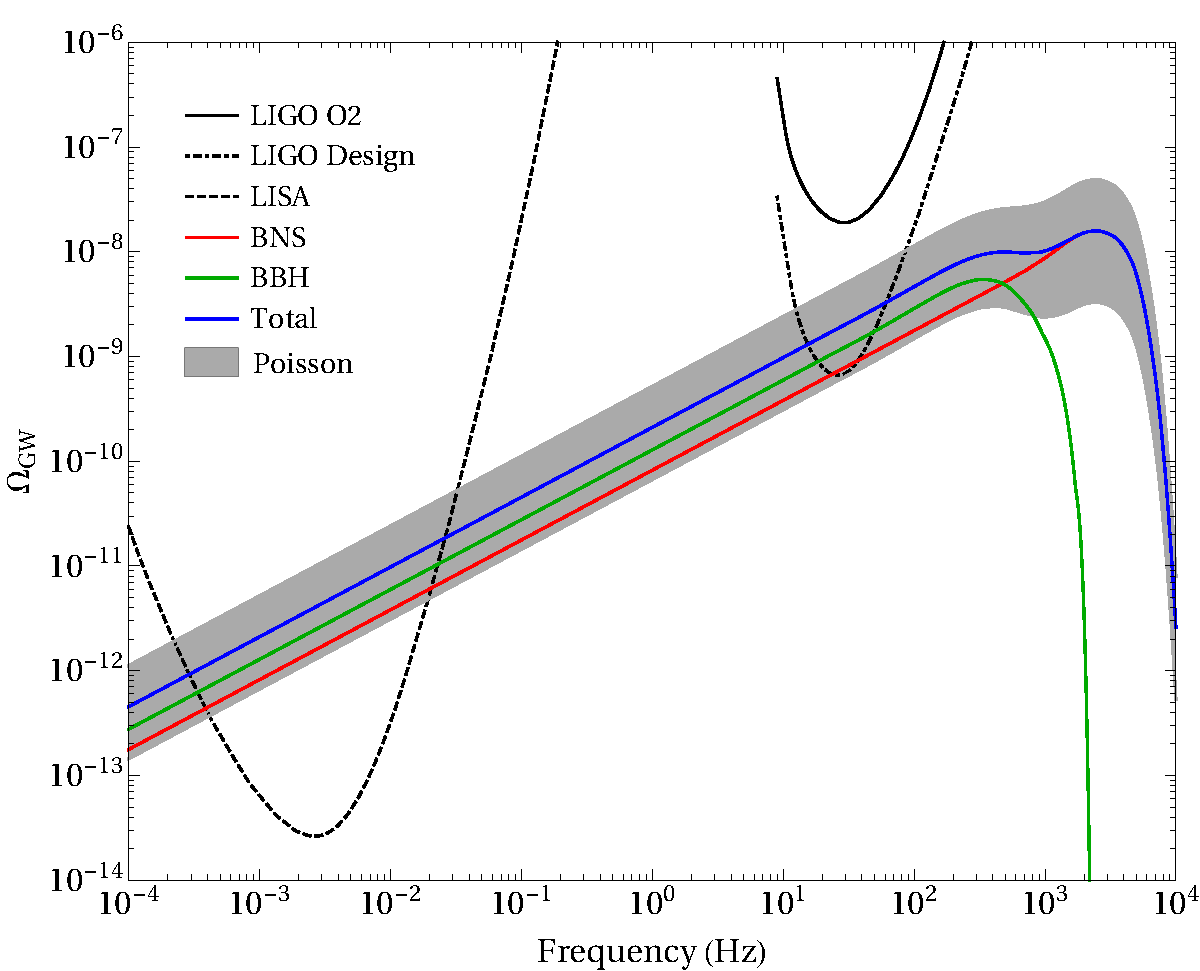
\includegraphics[width=\textwidth]{OmegaGW-sBH.pdf}
    \bicaption[来自天体物理双黑洞以及双中子星产生的随机引力波背景。绿线是双黑洞对应的随机引力波背景,而红线是双中子星对应的引力波背景。蓝色则表示总的随机引力波背景(包括双黑洞和双中子星的贡献);而灰色区域则表示总的引力波背景的泊松误差。在这里,我们取天体物理双黑洞的局域并合率为$R = 103_{-63}^{+110}$\,$\gpcyr$;而双中子星的局域并合率为$R = 1540_{-1220}^{+3200}$\,$\gpcyr$。图中的黑色实线表示LIGO第二个观测阶段的幂率积分曲线;点虚线表示LIGO设计阶段对应的幂率积分曲线;而虚线则表示LISA观测四年对应的幂率积分曲线。从图上可以看出,LIGO设计阶段和LISA对应的幂率积分曲线都能跨过泊松误差区域,表明天体物理双黑洞和双中子星产生的随机引力波背景可以被LIGO设计阶段和LISA探测到。]{\label{OmegaGW-sBH}
        来自天体物理双黑洞以及双中子星产生的随机引力波背景。绿线是双黑洞对应的随机引力波背景,而红线是双中子星对应的引力波背景。蓝色则表示总的随机引力波背景(包括双黑洞和双中子星的贡献);而灰色区域则表示总的引力波背景的泊松误差。在这里,我们取天体物理双黑洞的局域并合率为$R = 103_{-63}^{+110}$\,$\gpcyr$\citep{Abbott:2017vtc};而双中子星的局域并合率为$R = 1540_{-1220}^{+3200}$\,$\gpcyr$\citep{TheLIGOScientific:2017qsa}。图中的黑色实线表示LIGO第二个观测阶段的幂率积分曲线;点虚线表示LIGO设计阶段对应的幂率积分曲线;而虚线则表示LISA观测四年对应的幂率积分曲线。从图上可以看出,LIGO设计阶段和LISA对应的幂率积分曲线都能跨过泊松误差区域,表明天体物理双黑洞和双中子星产生的随机引力波背景可以被LIGO设计阶段和LISA探测到。
    }{The predicted stochastic gravitational-wave background from the binary neutron stars and stellar-origin binary black holes. 
    The red and green curves are backgrounds from the binary neutron stars (BNSs) and binary black holes (BBHs),
    respectively. 
    The total background is shown in the blue curve, while
    its Poisson error bars are in the grey shaded region.
    Here, we adopt the local merger rate $R = 103_{-63}^{+110}$\,$\gpcyr$ 
    for stellar-origin binary black holes \citep{Abbott:2017vtc},
    and $R = 1540_{-1220}^{+3200}$\,$\gpcyr$ for binary neutron stars
    \citep{TheLIGOScientific:2017qsa}.
    We also show the expected PI curves for LISA with $4$ years of 
    observation (dashed) and
    LIGO's observing runs of O2 (black) and design sensitivity (dot-dashed).
    The PI curves for LISA and LIGO's design sensitivity cross the Poisson
    error region, indicating the possibility to detect this background.}
\end{figure}

在估算并合率\Eq{sBHR}时,最复杂地方乃是计算天体物理黑洞和中子星的生成率。生成率可估算为\citep{Dvorkin:2016wac}
\e
    R_{\mathrm{birth}}(t,m_{\mathrm{rem}})=\int \psi [t-\tau(m_{*})] \phi(m_{*})
    \delta(m_{*}- g_{\mathrm{rem}}^{-1}(m_{\mathrm{rem}})) \text{d}m_{*},
\q
其中$m_{*}$为前身星的质量,$m_{\mathrm{rem}}$为最后天体的质量,而$\tau(m_{*})$前身星的寿命。$\tau(m_{*})$通常可以忽略\citep{Schaerer:2001jc}。上式中的$\phi(m_{*})$为初始质量函数(initial mass function,简称IMF)。对于中子星,初始质量函数为$1\,\Msun$到$2\,\Msun$之间的平坦分布;而对天体物理黑洞,初始质量函数$\phi(m_{*}) \propto m_{*}^{-2.35}$。此外,$\psi(t)$为恒星形成率(star formation rate,简称SFR),其为\citep{Nagamine:2003bd}
\e
\psi(z)= k \frac{a \exp[b(z-z_{m})]}{a-b+b \exp[a(z-z_{m})]}. 
\q
下面的计算中将使用文献\cite{Dvorkin:2016wac}给出的``\textit{Fiducial+PopIII}"模型的参数来计算上式。``\textit{Fiducial+PopIII}"是\textit{Fiducial}模型(其中$k=0.178 \Msun \mathrm{yr}^{-1} \mathrm{Mpc}^{-3}$,$z_{m}=2$, $a=2.37$,$b=1.8$)和\textit{PopIII}模型(其中$k=0.002 \Msun \mathrm{yr}^{-1} \mathrm{Mpc}^{-3}$,$z_{m}=11.87$,$a=13.8$,$b=13.36$)的综合。对于中子星,$g^{-1}_{\mathrm{ns}}(m_{\mathrm{ns}})=m_{\mathrm{ns}}$, 所以生成率的计算相对简单。而对于天体物理黑洞,其前身星的质量和最后残余质量存在特定的函数关系$m_{\mathrm{bh}}=g_{\mathrm{bh}}(m_{*})$。而这个函数关系是模型依赖的。在这里我们考虑``\textit{WWp}"模型\citep{Woosley:1995ip}。这个模型和广为使用的``\textit{Fryer}"模型\citep{Dvorkin:2016wac}在低红移时是不可区分的,但足够简单。对于初始质量为$m_{*}$的前身星,其残余的黑洞质量$m_{\mathrm{bh}}$为
\e
\frac{m_{\mathrm{bh}}}{m_{*}}=A \left(\frac{m_{*}}{40\Msun} \right)^{\beta} \frac{1}{\left( \frac{Z(z)}{0.01 Z_\odot} \right)^{\gamma} +1},
\q
其中$Z(z)$为金属丰度,其具体的函数形式由文献\cite{Belczynski:2016obo}给出。上式中各个参数的取值为$A=0.3$,$\beta =0.8$和$\gamma =0.2$ \citep{Dvorkin:2016wac}。通过解以上方程,就能得到$m_{*} = g_{\mathrm{bh}}^{-1}(m_{\mathrm{bh}})$。

\begin{table}[htb!]
    \centering
    \begin{tabular}{c|c|c}
        &\ $\Omega_{\mathrm{GW}}(25 \, \mathrm{Hz})$ \
        &\ $\Omega_{\mathrm{GW}}(3 \times 10^{-3} \, \mathrm{Hz})$\,\\
        \hline
        BNS\, &  $0.7^{+1.5}_{-0.6} \times 10^{-9}$ 
        & $1.7^{+3.5}_{-1.4} \times 10^{-12}$ \\
        [.3em]
        \hline
        BBH\, & $1.1^{+1.2}_{-0.7} \times 10^{-9}$  
        & $2.7^{+2.8}_{-1.6} \times 10^{-12}$ \\
        [.3em]
        \hline
        Total\, & $1.8^{+2.7}_{-1.3} \times 10^{-9}$  
        & $4.4^{+6.3}_{-3.0} \times 10^{-12}$ \\
        [.2em]
    \end{tabular}
    \bicaption{\label{Omegaf-sBH}
        天体物理双黑洞产生的随机引力波背景、双中子星产生的随机引力波背景以及总的随机引力波背景在LIGO和LISA最灵敏的频率附近(分别为$25 \, \mathrm{Hz}$和$3 \times 10^{-3} \, \mathrm{Hz}$)的大小。我们还给出了$90\%$的泊松误差范围。
    }{Estimates of the background energy density $\ogw (\nu)$ at the most
    sensitive frequencies of LIGO (near $25$ Hz) and LISA 
    (near $3\times 10^{-3}$ Hz) for each of the binary neutron star (BNS), stellar-origin binary black hole (BBH) and total background contributions, along with the $90\%$ Poisson error bounds.}
\end{table}


\begin{figure}[htb!]
    \centering
    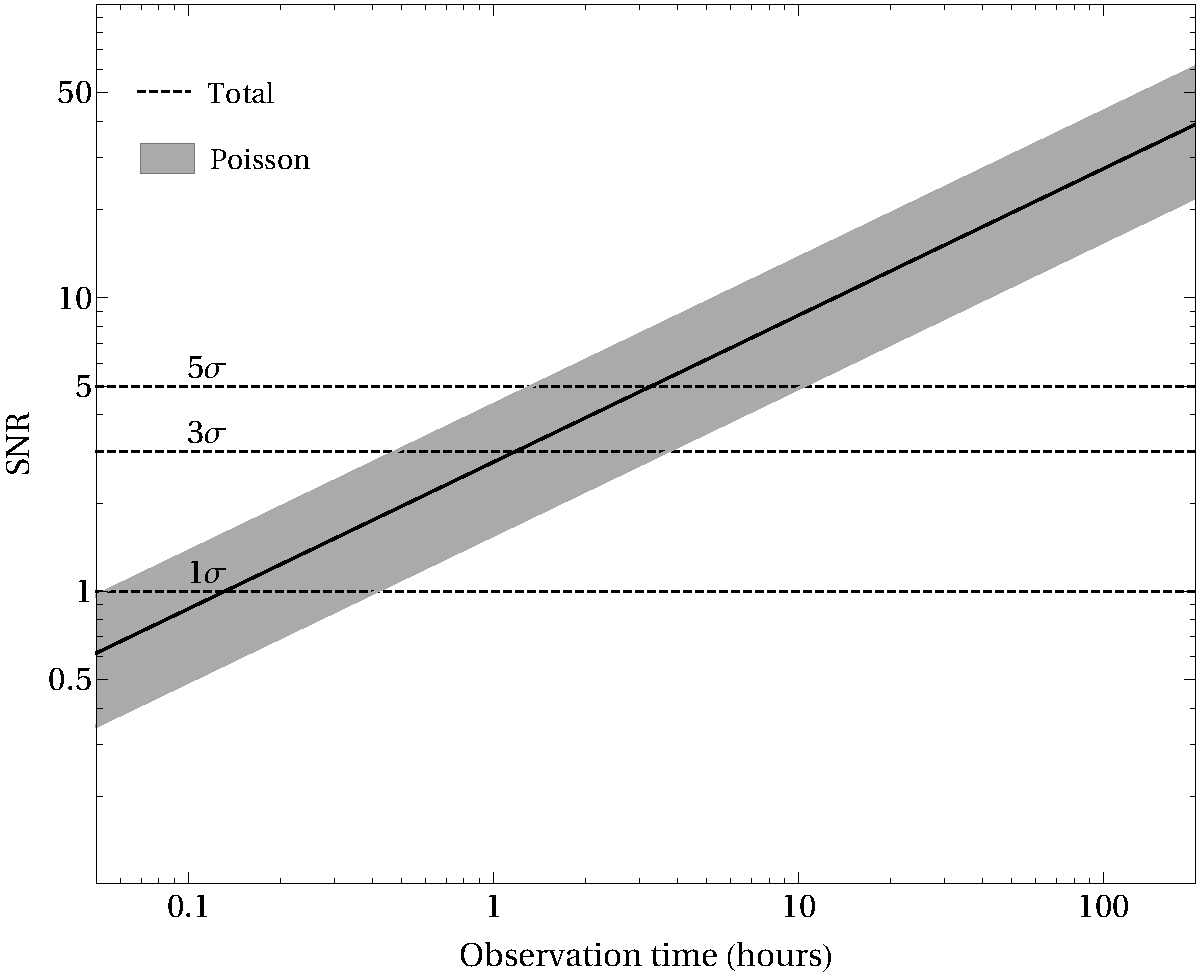
\includegraphics[width=\textwidth]{SNR-sBH.pdf}
    \bicaption[LISA探测器对探测天体物理双黑洞和双中子星产生的总的随机引力波背景的信噪比随观测时间的关系。黑色实线表示信噪比的中心值,而灰色区域表示信噪比的误差范围。在这里,我们取天体物理双黑洞的局域并合率为$R = 103_{-63}^{+110}$\,$\gpcyr$;而双中子星的局域并合率为$R = 1540_{-1220}^{+3200}$\,$\gpcyr$。在大约观测$20$个小时后,LISA可以探测到中心值大小的总的随机引力波背景;探测的信噪比为$\mathrm{SNR}=5$。]{\label{SNR-sBH} 
        LISA探测器对探测天体物理双黑洞和双中子星产生的总的随机引力波背景的信噪比随观测时间的关系。黑色实线表示信噪比的中心值,而灰色区域表示信噪比的误差范围。在这里,我们取天体物理双黑洞的局域并合率为$R = 103_{-63}^{+110}$\,$\gpcyr$\citep{Abbott:2017vtc};而双中子星的局域并合率为$R = 1540_{-1220}^{+3200}$\,$\gpcyr$\citep{TheLIGOScientific:2017qsa}。在大约观测$20$个小时后,LISA可以探测到中心值大小的总的随机引力波背景;探测的信噪比为$\mathrm{SNR}=5$。
    }{The SNR of LISA as a function of observing time for median total 
    stochastic gravitational-wave background (black curve) and associated uncertainties (grey shaded region),
    from the stellar-origin binary black holes and binary neutron stars.
    Here, we adopt the local merger rate $R = 103_{-63}^{+110}$\,$\gpcyr$ 
    for stellar-origin binary black holes \citep{Abbott:2017vtc},
    and $R = 1540_{-1220}^{+3200}$\,$\gpcyr$ for binary neutron stars
    \citep{TheLIGOScientific:2017qsa}.
    The predicted median total background can be detected with 
    $\mathrm{SNR}=5$ after about $20$ hours of observation time.}
\end{figure}

\begin{figure}[htb!]
    \centering
    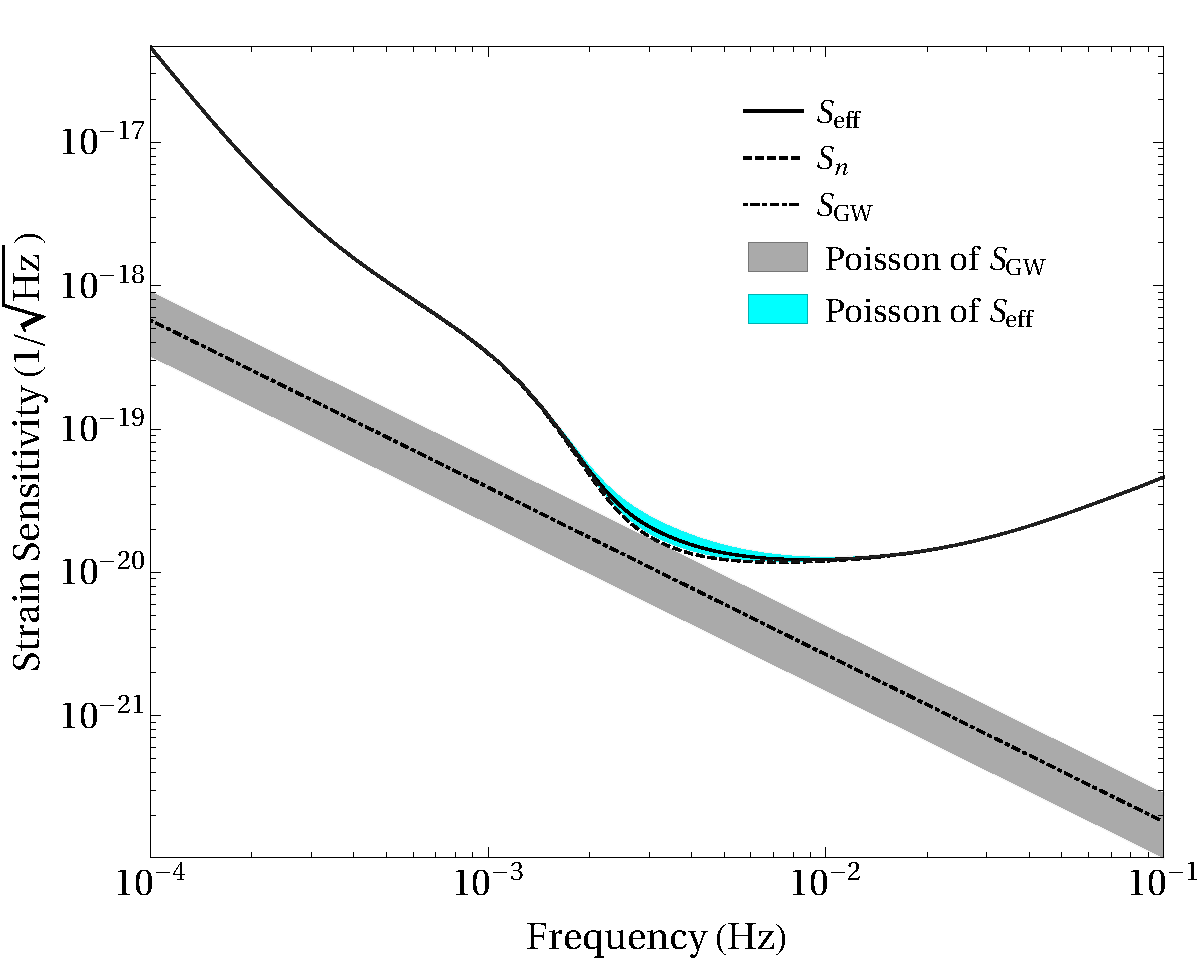
\includegraphics[width=\textwidth]{lisa-sensitivity-sBH.pdf}
    \bicaption{\label{lisa-sensitivity-sBH}
        由天体物理双黑洞和双中子星产生的总的随机引力波背景导致LISA探测器的有效应变灵敏度$S_{\mathrm{eff}}$(黑色实线)以及相应的泊松误差(青色区域)。图中还给出了LISA探测器的应变灵敏度$S_n$(虚线)以及随机引力波背景对应的应变灵敏度$S_{\mathrm{GW}}$(点虚线)和相应的泊松误差(灰色区域)。
    }{The effective strain sensitivity $S_{\mathrm{eff}}$ (black solid curve) of LISA and its Poisson uncertainties (cyan region), due to the effect of the total stochastic gravitational-wave background from stellar-origin binary black holes and binary neutron stars. We also show LISA's strain sensitivity $S_n$ (dashed curve), and $S_{\mathrm{GW}}$ (dot-dashed curve) along with its Poisson uncertainties (grey shaded region).}
\end{figure} 

\begin{figure}[htbp!]
    \centering
    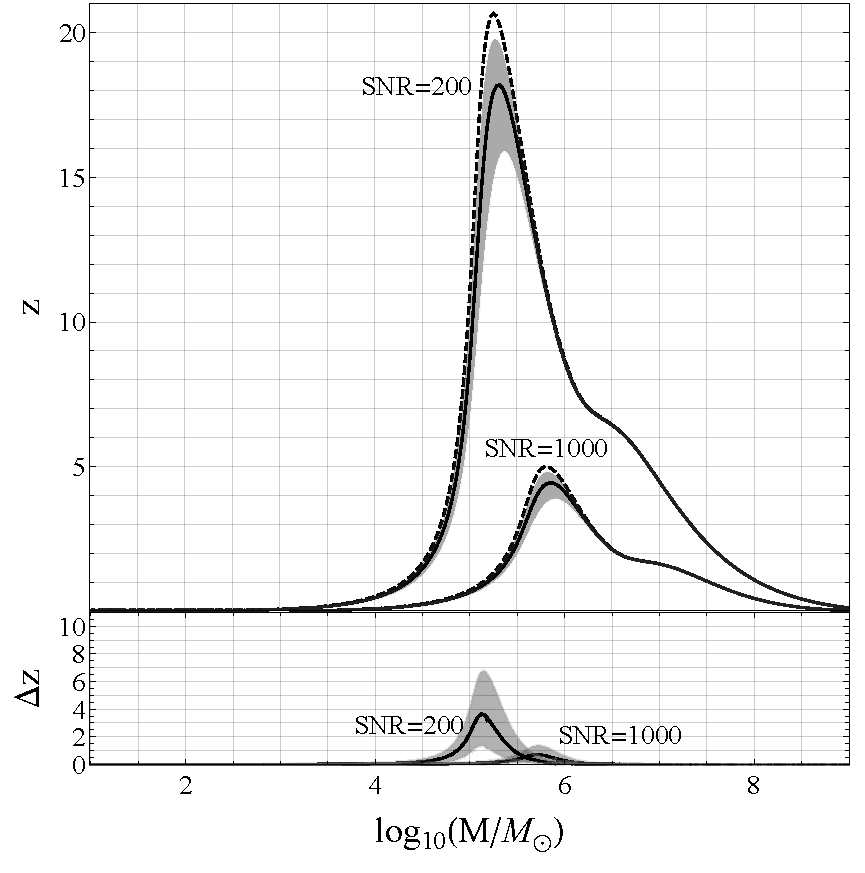
\includegraphics[width=\textwidth]{z-sBH.pdf}
    \bicaption[由天体物理双黑洞和双中子星产生的总的随机引力波背景对LISA探测器对于大质量双黑洞系统最大可探测红移$z$的影响。我们用$M$表示大质量双黑洞的总质量。我们固定质量比为$q=0.2$。我们分别考虑$\SNR=200$和$\SNR=1000$的两种情况。上图的虚线表示LISA最大可探测红移的等高线,而黑色实线表示考虑了随机引力波背景后LISA的最大可探测红移的等高线。灰色区域是黑色实线对应的泊松误差范围。下图给出了考虑随机引力波背景后对LISA最大可探测红移所引起的变化及误差范围。]{\label{z-sBH}
        由天体物理双黑洞和双中子星产生的总的随机引力波背景对LISA探测器对于大质量双黑洞系统最大可探测红移$z$的影响。我们用$M$表示大质量双黑洞的总质量。仿照\cite{Audley:2017drz},我们固定质量比为$q=0.2$。我们分别考虑$\SNR=200$和$\SNR=1000$的两种情况。上图的虚线表示LISA最大可探测红移的等高线,而黑色实线表示考虑了随机引力波背景后LISA的最大可探测红移的等高线。灰色区域是黑色实线对应的泊松误差范围。下图给出了考虑随机引力波背景后对LISA最大可探测红移所引起的变化及误差范围。
    }{The impacts of the total stochastic gravitational-wave background from stellar-origin binary black holes and binary neutron stars 
        on the largest detectable redshift $z$ of MBHB (with total mass $M$) coalescences for LISA.
        The mass ratio is set to $q=0.2$ following \cite{Audley:2017drz}. 
        The upper panel shows the contours of $\SNR=200$ and $\SNR=1000$ 
        for LISA (dashed curves), 
        together with the effect of stochastic gravitational-wave background (black curves) and the Poisson error 
        bars (grey shaded region). 
        The lower panel shows the residuals of corresponding contours. }
\end{figure}

对并合率密度中的质量做积分,即可得到并合率随红移的演化函数
\e
\mR(z)  =\int \mR(z,m_{1},m_{2} )\, \rmd m_{1} \text{d}m_{2}.
\q
对于天体物理双黑洞,引力波对其局域并合率$R \equiv \mR(z=0)$的限制为$R = 103_{-63}^{+110}$\,$\gpcyr$\citep{Abbott:2017vtc};而对于双子星,引力波的限制为$R = 1540_{-1220}^{+3200}$\,$\gpcyr$\citep{TheLIGOScientific:2017qsa}。利用公式\Eq{OmegaGW},我们就可以计算来自天体物理双黑洞以及双中子星产生的随机引力波背景。在\Fig{OmegaGW-sBH}中,我们给出了相应的随机引力波背景的能量密度谱。为了和引力波实验观测数据比较,我们还画出了LIGO探测器\citep{TheLIGOScientific:2017qsa}的幂率积分(power-law integrated,简称PI)曲线和LISA探测器\citep{Cornish:2017vip,Cornish:2018dyw}的幂率积分曲线。结果表明,不管是天体物理双黑洞产生的引力波背景还是双中子星产生的引力波背景,在未来都很可能被LIGO和LISA探测到。另外,在LIGO和LISA的可探测频段内,天体物理双黑洞和双中子星产生的引力波背景都近似和频率的$2/3$次方成正比,即$\ogw \propto \nu^{2/3}$。这是因为在可探测的频段内,随机引力波背景的贡献主要来自于双黑洞或双中子星的旋进阶段,而在旋进阶段,单个双黑洞或双中子星辐射的引力波能量谱大概就和频率的$2/3$次方成正比。在\Table{Omegaf-sBH}中,我们总结了在LIGO和LISA最灵敏的频率附近的随机引力波背景的能量密度的大小$\ogw (\nu)$。对于LIGO探测器来说,其最灵敏的频率大概是$25$Hz左右,而LISA探测器最灵敏的频率大概是$3\times 10^{-3}$Hz左右。


对于LISA探测器,假如其观测时间为$T$,其所能观测到随机引力波背景的信噪比(signal-to-noise ratio,简称SNR)为\citep{Thrane:2013oya,Caprini:2015zlo}
\e
\text{SNR}=\sqrt{T} \left[ \int \rmd \nu \frac{\Omega_{\mathrm{GW}}(\nu)}{\Omega_{n}(\nu)} \right] ^{1/2},
\q
其中$\Omega_{n}(\nu)$定义为
\e 
\Omega_{n}(\nu)\equiv 2 \pi^2 \nu^3 S_{n}(\nu)/\left(3 H_{0}^2 \right),
\q 
而$S_{n}$为LISA的噪音应变灵敏度。\Fig{SNR-sBH}给出了预期累积信噪比关于时间的函数关系。由图可知,在观测$20$小时后,LISA可以探测到来自天体物理双黑洞和双中子星的中心值大小的随机引力波背景,相应的信噪比为$\mathrm{SNR} = 5$。在最乐观的情况下LISA观测$5$个小时就能探测到信噪比$\mathrm{SNR} = 5$的总的随机引力波背景,而在最悲观的情况下LISA观测$8$天能探测到信噪比$\mathrm{SNR} = 5$的总的随机引力波背景。

由以上分析可知,如果不在LISA的噪音背景中把来自天体物理双黑洞和双中子星产生的总的随机引力波背景扣除掉,这些引力波背景可能成为LISA新的噪音源,从而影响LISA的科学探测目标。例如,对于LISA来说,探测大质量双黑洞(massive black hole binary,简称MBHB)的并合是LISA的一个关键科学目标\citep{Audley:2017drz},而如果不把这些引力波背景从噪音中扣除掉的话,会降低LISA对于大质量双黑洞的最大可探测红移。 


仿照\cite{Barack:2004wc,Cornish:2018dyw},我们定义随机引力波背景产生的等效噪音应变灵敏度为
\e
S_{\mathrm{GW}}(\nu) \equiv \frac{3 H_{0}^2}{2 \pi^2}
\frac{\Omega_{\mathrm{GW}}(\nu)}{\nu^3}.
\q
将随机引力波背景产生的等效噪音应变灵敏度加到LISA的噪音应变灵敏度$S_{n}(\nu)$中,即可得到有效的总的应变灵敏度$S_{\mathrm{eff}}(\nu)$,即
\e 
S_{\mathrm{eff}}(\nu)=S_{n}(\nu)+S_{\mathrm{GW}}(\nu).
\q
在\Fig{lisa-sensitivity-sBH}中,我们给出了相应的应变灵敏度曲线。对于探测单个源传播过来的引力波应变信号(也就是通常说的波形)$h(t)$,LISA对应的信噪比为
\e
\SNR = 2 \left[ \int \rmd \nu 
\frac{|\tilde{h}(\nu)|^2}{S_{\mathrm{eff}}(\nu)} \right]^{1/2},
\q
其中$\tilde{h}(\nu)$是$h(t)$在频率空间的波形。在这里我们使用\cite{Ajith:2007kx}给出的唯象波形来描述大质量双黑洞系统产生的引力波。

对于LISA来说,研究大质量黑洞的增长机制是其重要的科学探索目标之一\citep{Audley:2017drz}。为了实现这一目标,要求LISA对大质量黑洞无量纲自旋的探测的绝对误差要小于$0.1$,并且探测到的自旋方向的误差要小于$10^{\circ}$。为了达到这些要求,需要探测的信噪比达到$200$以上。在这里我们考虑了$\SNR=200$和$\SNR=1000$的两种情况。\Fig{z-sBH}给出了随机引力波背景对LISA探测大质量双黑洞并合的信噪比的影响,表明最大可探测红移会由于未解析出来的随机引力波背景的影响而减小。这也表明LISA可探测的区域被压低了,从而减少LISA可探测到的大质量双黑洞并合的事件数。目前的研究表明,为了形成大质量黑洞通常需要种子黑洞的质量在$10^3 \Msun$到$10^5 \Msun$的量级,而且相应的红移在在$10\lesssim z \lesssim 15$\citep{Volonteri:2010wz}。从\Fig{z-sBH}看出,由于随机引力波背景导致的等效噪音可以压低LISA对$10^5 \Msun$以上的种子黑洞并合的最大可探测红移。因此,为了提高LISA探测器的探测灵敏度,需要设法将这些随机引力波背景从背景噪音中扣除掉。

%%%%%%%%%%%%%%%%%%%%%%%%%%%%%%%%%%%%%%%%%%%%%%%%%%%%%%%%%%%%%%%%%%%%%%
\section{\label{PBH}原初双黑洞产生的随机引力波背景}
在本节中,我们将计算原初双黑洞产生的随机引力波背景。我们假设\lvc 目前所探测到的所有双黑洞都来自原初黑洞。
在这里,我们使用文献\cite{Chen:2018czv}给出的原初双黑洞的并合率,也就是我们在上一章所推导出来的并合率表达式。在计算并合率时,我们考虑了所有原初黑洞和线性密度扰动对原初双黑洞角动量的贡献。对于一个一般的已经归一化的原初黑洞质量概率分布函数$P(m|\vth)$,其共动并合率密度分布为\citep{Chen:2018czv}
\m\label{calR2} 
\mR_{12}(t|\vth) & \app & 3.9\cdot 10^6\times \({t\over t_0}\)^{-{34\over 37}} f^2 (f^2+\sigma_{\mathrm{eq}}^2)^{-{21\over 74}} (m_1 m_2)^{{3\over 37}} (m_1+m_2)^{36\over 37} \nonumber \\
&& \times  \min\(\frac{P(m_1|\vth)}{m_1}, \frac{P(m_2|\vth)}{m_2}\) \({P(m_1|\vth)\over m_1}+{P(m_2|\vth)\over m_2}\),
\n
其中$\vth$是质量函数中所带有的参数,$t_0$为宇宙年龄。需要注意的是,上式的并合率密度的单位为$\gpcyr$。此外,$\sigma_{\mathrm{eq}}$是其余暗物质在辐射-物质平衡时期在${\cal O}(10^0\sim10^3) M_\odot$尺度上的密度扰动的方差。类似于\cite{Ali-Haimoud:2017rtz,Chen:2018czv},我们取$\sigma_{\mathrm{eq}}\approx 0.005$。而且原初黑洞的质量$m_1$和$m_2$都是以$\Msun$为单位的。在这里$f$是总原初黑洞占非相对论物质的丰度,其和原初黑洞占冷暗物质的丰度$\fpbh$的关系为$\fpbh\equiv \Omega_{\mathrm{PBH}}/\Omega_{\mathrm{CDM}} \approx f/0.85$。

对并合率密度分布\eqref{calR2}的质量做积分,即可得到并合率随时间或红移的演化
\e
\mR(t|\vth) = \int \mR_{12}(t|\vth)\ \rmd m_1\, \rmd m_2.
\q 
由此可以得到局域的并合率密度分布
\e 
\mR_{12}(t_0|\vth) = R\, p(m_1,m_2|\vth),
\q 
其中$p(m_1,m_2|\vth)$为并合双黑洞中黑洞质量的概率分布,而局域并合率$R \equiv \mR(t_0|\vth)$是一个归一化系数。由定义可知,$p(m_1,m_2|\vth)$满足归一化条件,即
\e 
 \int p(m_1,m_2|\vth) \rmd m_1\, \rmd m_2 = 1.
\q 
需要注意的是,这里的质量是源参考系的质量,而不是探测器参考系的质量。

下面我们需要将理论得到的原初双黑洞的并合率和引力波实验数据做拟合,从而推断出模型参数$\{\vth, R\}$的取值。在这里我们不需用用到\lvc 最原始的应变数据,而只需要用到\lvc 公布的双黑洞并合事件的后验分布数据,然后用到层次贝叶斯推断(hierarchical Bayesian inference)的方法去做模型的参数估计。层次贝叶斯推断方法的优点是可以节省大量的计算量。这一方法已经被广泛应用于引力波领域\citep{Abbott:2016nhf,Abbott:2016drs,TheLIGOScientific:2016pea,Wysocki:2018mpo,Fishbach:2018edt,Mandel:2018mve,Thrane:2018qnx}。下面简单介绍这一方法。假定已有$N$个双黑洞并合事件的数据$\vd = (d_1, \dots, 
d_N)$,那么由理论模型得到数据的似然函数(likelihood function)为\citep{Wysocki:2018mpo,Fishbach:2018edt,Mandel:2018mve,Thrane:2018qnx}
\e\label{likelihood1}
p(\vd|\vth, R) \propto R^{N} e^{-R\, \beta(\vth)} \prod_i^N 
\int \rmd\vla\ p(d_i|\vla)\ p(\vla|\vth),
\q 
其中$\vla \equiv \{m_1, m_2\}$。在上式中$p(d_i|\vla)$为单个引力波事件在给定双黑洞参数$\vla$时得到数据$d_i$的似然函数。由于\lvc 在分析单个引力波事件时,其用到的黑洞的质量参数的先验分布(prior distribution)为平的分布,所以对于单个事件而言,其似然函数$p(d_i|\vla)$和后验分布成正比$p(\vla|d_i)$,即$p(d_i|\vla) \propto p(\vla|d_i)$。因此我们可以直接用\lvc 公开的每个双黑洞并合事件的后验分布\citep{Vallisneri:2014vxa,TheLIGOScientific:2016pea,Biwer:2018osg}来计算\Eq{likelihood1}的积分。同时,\Eq{likelihood1}的$\beta(\vth)$定义为
\e 
\beta(\vth) \equiv \int \rmd\vla\ VT(\vla)\ p(\vla|\vth),
\q 
其中$VT(\vla)$为\lvc 可探测的时空体积。我们用半解析的方法\cite{Abbott:2016nhf,Abbott:2016drs}来计算$VT$。在这里我们忽略了黑洞的自旋效应,并且使用``早期高灵敏度”(``Early High Sensitivity")的噪音功率谱(power spectral density, 简称PSD)来近似LIGO的前两个观测阶段的噪音功率谱。我们取单个引力波探测器的信噪比为$\SNR = 8$作为探测到引力波事件的阀值。真实的LIGO探测器是由两个探测器组成的引力波探测器网络。对于整个探测器网络来说,相应的信噪比阀值大约是$12$。

给定先验分布$p(\vth, R)$后,我们就能得到对应的后验分布
\e\label{post1} 
p(\vth, R|\vd) \propto p(\vd |\vth, R)\ p(\vth, R).
\q 
对于$\vth$参数我们选平的分布,而对于局域并合率$R$我们选对数平的分布。换言之,我们假定的先验分布为
\e 
p(\vth, R) \propto \frac{1}{R}.
\q 
有了先验分布,再利用似然函数\eqref{likelihood1}式,我们可以得到对局域并合率$R$做边际化后的后验分布,即
\e\label{post_vth1} 
p(\vth|\vd) \propto \[\beta(\vth)\]^{-N} 
\prod_i^N \int \rmd\vla\ p(d_i|\vla)\ p(\vla|\vth).
\q
这个后验分布公式已经被广泛应用于引力波的参数推断中\citep{Abbott:2016nhf,Abbott:2017vtc,TheLIGOScientific:2016pea,Abbott:2016drs,Fishbach:2017zga}。我们将仿照文献\cite{Abbott:2016nhf,TheLIGOScientific:2016pea,Abbott:2016drs,Abbott:2017vtc}的做法,先用\Eq{post_vth1}来限制$\vth$参数,然后在\Eq{post1}中将$\vth$固定成最佳拟合值来估计局域并合率$R$的值。和\ref{SBH}小节一样,我们考虑的双黑洞的质量范围为$5\Msun \leq m_2 \leq m_1$且$m_1 + m_2 \leq 100\Msun$。这里我们只用LIGO第一个观测阶段观测到的$3$个双黑洞并合事例来拟合模型参数。LIGO的第一个观测阶段观测的有效时间为$48.6$天\citep{TheLIGOScientific:2016pea}。在\Table{events2}中,我们列出了这$3$个双黑洞并合事件的源的主要性质。

%%%%%%%%%%%%%%%%%%%%%%%%%%%%%%%%%%%%%%%%%%%%%%%%%%%%%%%%%%%%%%%%%%%%%%
\begin{table}[htb!]
    \centering
    \begin{tabular}{c|c|c|c}
        事件 & 较重黑洞的质量 & 较轻黑洞的质量 & 红移\\
        \hline
        GW150914\, 
        &  $36.2\,^{+5.2}_{-3.8}$\,$\Msun$ & $29.1\,^{+3.7}_{-4.4}$\,$\Msun$ 
        & $0.09\,^{+0.03}_{-0.04}$\\
        [.3em]
        \hline
        LVT151012\, 
        & $23\,^{+18}_{-6}$\,$\Msun$  & $13\,^{+4}_{-5}$\,$\Msun$ 
        & $0.20\,^{+0.09}_{-0.09}$\\
        [.3em]
        \hline
        GW151226\, 
        &  $14.2\,^{+8.3}_{-3.7}$\,$\Msun$  & $7.5\,^{+2.3}_{-2.3}$\,$\Msun$ 
        & $0.09\,^{+0.03}_{-0.04}$\\
        [.3em]
        \hline
    \end{tabular}
    \bicaption[\lvc 第一个观测阶段探测到的$3$个双黑洞并合事件的源的主要性质。]{\lvc 第一个观测阶段探测到的$3$个双黑洞并合事件的源的主要性质\citep{Abbott:2016blz,TheLIGOScientific:2016pea,TheLIGOScientific:2016qqj,TheLIGOScientific:2016pea,Abbott:2016nmj}。
    }{A summary of the masses and source redshifts of the $3$ 
    binary black holes detected by \lvc\, collaborations
    ~\citep{Abbott:2016blz,TheLIGOScientific:2016pea,TheLIGOScientific:2016qqj,TheLIGOScientific:2016pea,Abbott:2016nmj}.}
    \label{events2}
\end{table}
%%%%%%%%%%%%%%%%%%%%%%%%%%%%%%%%%%%%%%%%%%%%%%%%%%%%%%%%%%%%%%%%%%%%%%

在以下的两个小节中我们将考虑两种不同的原初黑洞的质量分布函数。我们先用LIGO的引力波数据来限制模型参数$\{\vth, R\}$,然后由此计算相应的随机引力波背景。

%%%%%%%%%%%%%%%%%%%%%%%%%%%%%%%%%%%%%%%%%%%%%%%%%%%%%%%%%%%%%%%%%%%%%%
\subsection{幂率质量函数}
这里我们考虑幂率形式的原初黑洞质量分布函数\citep{Carr:1975qj}
\e\label{power}
P(m)\approx {\alpha-1\over \Mmin} \({m\over \Mmin}\)^{-\alpha},
\q
其中$m\geq \Mmin = 5\Msun$,且要求幂指数$\alpha>1$。在这种情况下,模型有两个自由参数,为$\{\vth, R\} = \{\al, R\}$。

\begin{figure}[htb!]
    \centering
    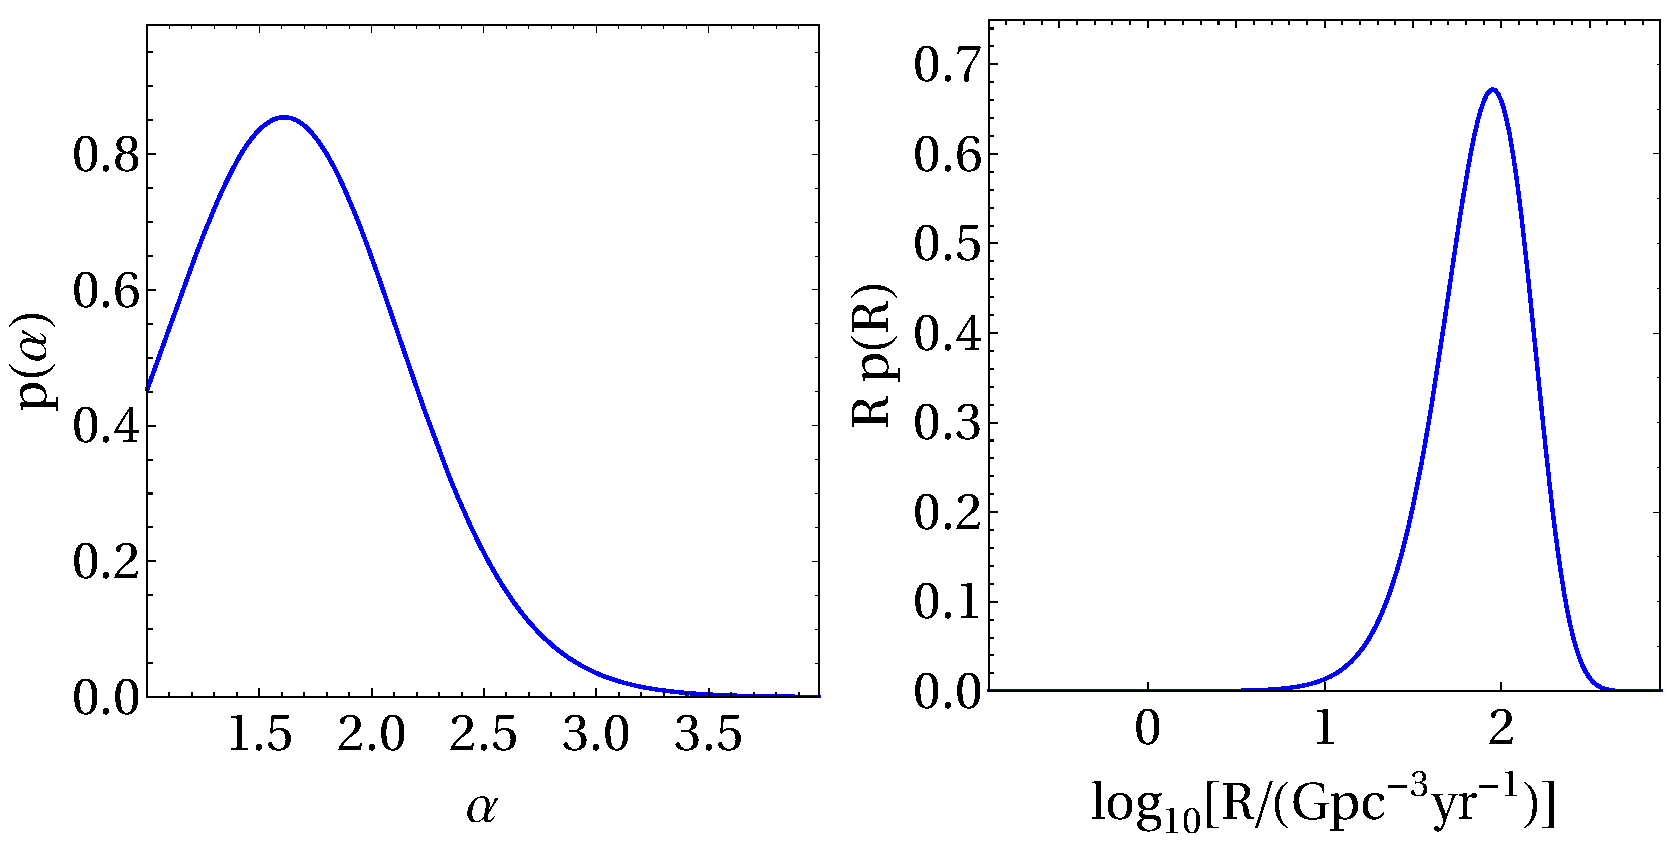
\includegraphics[width=\textwidth]{posterior-PBH-power.pdf}
    \bicaption{\label{posterior-PBH-power} 
        当原初黑洞质量函数为\textit{幂率}形式的情况下,用LIGO第一个观测阶段的$3$个双黑洞并合事件拟合得到模型参数$\{\vth, R\} = \{\al, R\}$的后验分布。
    }{The posterior distributions for $\{\vth, R\} = \{\al, R\}$ for
    \textit{power-law} mass function of PBHs, by using $3$ events from 
    LIGO's O1 observing run.}
\end{figure}

\begin{figure}[htbp!]
    \centering
    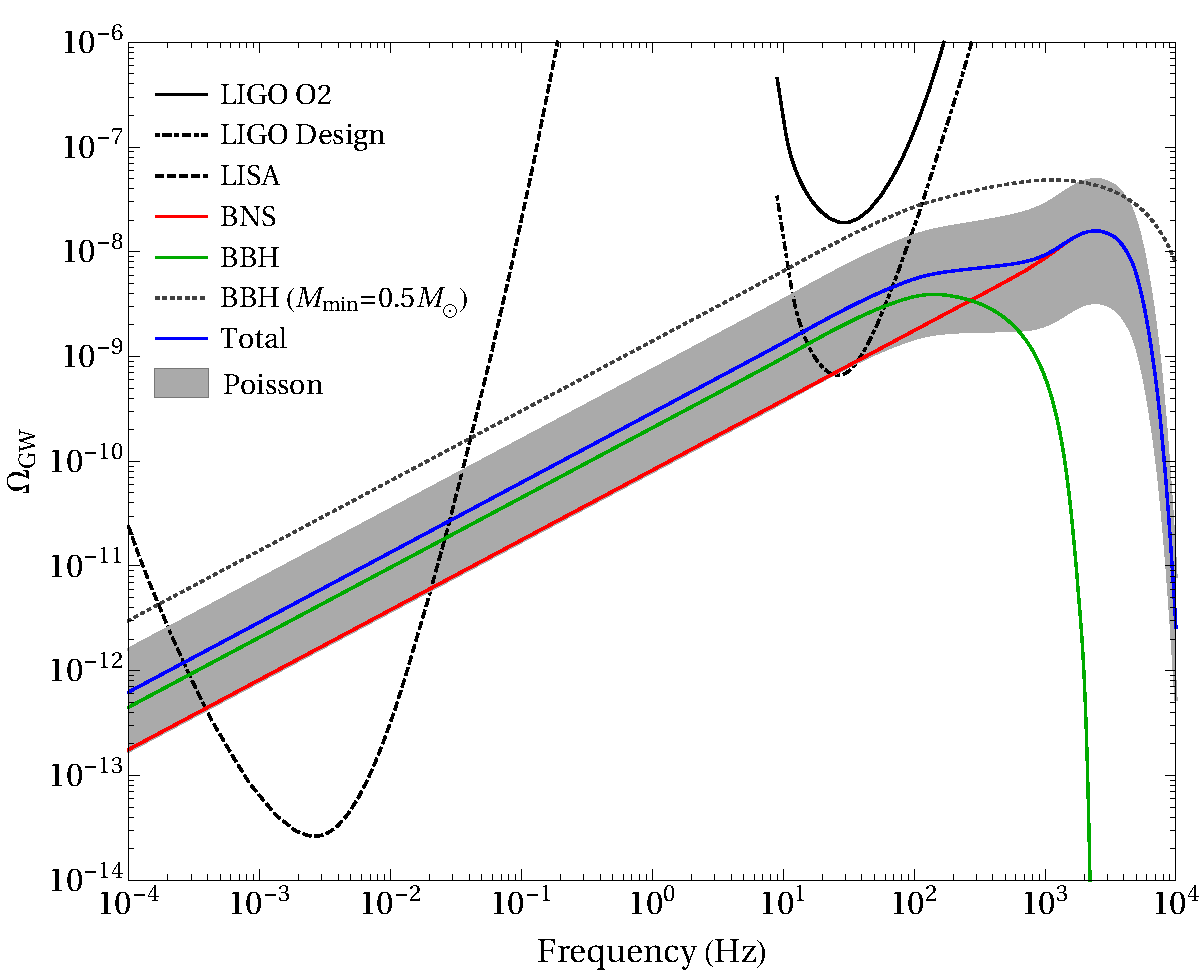
\includegraphics[width=0.8\textwidth]{OmegaGW-PBH-power.pdf}
    \bicaption[来自幂率质量分布的原初双黑洞以及双中子星产生的随机引力波背景。绿线是双黑洞对应的随机引力波背景,而红线是双中子星对应的随机引力波背景。蓝色表示总的随机引力波背;而灰色区域表示总的随机引力波背景的泊松误差。对于双黑洞,我们固定$\al$和局域并合率$R$为其最佳拟合值,即$\al = 1.61$和$R = 80\,^{+108}_{-56}$\, $\gpcyr$,且$\fpbh = 3.8\,^{+2.3}_{-1.8} \times 10^{-3}$。而对于双中子星,我们取局域并合率为$R = 1540_{-1220}^{+3200}$\,$\gpcyr$。图中的黑色实线表示LIGO第二个观测阶段(O2)的幂率积分曲线;点虚线表示LIGO设计阶段对应的幂率积分曲线;而虚线则表示LISA观测四年对应的幂率积分曲线。从图上可以看出,LIGO设计阶段和LISA对应的幂率积分曲线都能跨过泊松误差区域,表明原初双黑洞和双中子星产生的随机引力波背景可以被LIGO设计阶段和LISA探测到。]{\label{OmegaGW-PBH-power} 
        来自幂率质量分布的原初双黑洞以及双中子星产生的随机引力波背景。绿线是双黑洞对应的随机引力波背景,而红线是双中子星对应的随机引力波背景。蓝色表示总的随机引力波背;而灰色区域表示总的随机引力波背景的泊松误差。对于双黑洞,我们固定$\al$和局域并合率$R$为其最佳拟合值,即$\al = 1.61$和$R = 80\,^{+108}_{-56}$\, $\gpcyr$。该情况下对应的原初黑洞占暗物质的丰度为$\fpbh = 3.8\,^{+2.3}_{-1.8} \times 10^{-3}$。而对于双中子星,我们取局域并合率为$R = 1540_{-1220}^{+3200}$\,$\gpcyr$\citep{TheLIGOScientific:2017qsa}。图中的黑色实线表示LIGO第二个观测阶段(O2)的幂率积分曲线;点虚线表示LIGO设计阶段对应的幂率积分曲线;而虚线则表示LISA观测四年对应的幂率积分曲线。从图上可以看出,LIGO设计阶段和LISA对应的幂率积分曲线都能跨过泊松误差区域,表明原初双黑洞和双中子星产生的随机引力波背景可以被LIGO设计阶段和LISA探测到。
    }{The predicted stochastic gravitational-wave background from the binary neutron stars (BNSs)) and primordial-origin binary black holes (BBHs)
    with a \textit{power-law} mass function. 
    The red and green curves are backgrounds from the binary neutron stars and binary black holes, respectively. 
    The total background is shown in the blue curve, while
    its Poisson error bars are in the grey shaded region.
    For binary black holes, we adopt the best-fit value for $\al = 1.61$, 
    and the inferred local merger rate $R = 80\,^{+108}_{-56}$\, $\gpcyr$,
    which corresponds to $\fpbh = 3.8\,^{+2.3}_{-1.8} \times 10^{-3}$. 
    And for binary neutron stars, we adopt $R = 1540_{-1220}^{+3200}$\,$\gpcyr$ 
    \citep{TheLIGOScientific:2017qsa}.
    The dotted line shows the background from binary black holes with $\Mmin = 0.5 \Msun$, 
    by fixing $\al = 1.61$ and $R = 80$\, $\gpcyr$.
    We also show the expected PI curves for LISA with $4$ years of 
    observation (dashed) and
    LIGO's observing runs of O2 (black) and design sensitivity (dot-dashed).
    The PI curves for LISA and LIGO's design sensitivity cross the Poisson
    error region, indicating the possibility to detect this background.}
\end{figure}

\begin{table}[htb!]
    \centering
    \begin{tabular}{c|c|c}
        &\ $\Omega_{\mathrm{GW}}(25 \, \mathrm{Hz})$ \
        &\ $\Omega_{\mathrm{GW}}(3 \times 10^{-3} \, \mathrm{Hz})$\,\\
        \hline
        BNS\, &  $0.7^{+1.5}_{-0.6} \times 10^{-9}$ 
        & $1.7^{+3.5}_{-1.4} \times 10^{-12}$ \\
        [.3em]
        \hline
        BBH\, & $1.8_{-1.3}^{+2.5} \times 10^{-9}$  
        & $4.3^{+5.9}_{-3.0} \times 10^{-12}$ \\
        [.3em]
        \hline
        Total\, & $2.5^{+4.0}_{-1.9} \times 10^{-9}$  
        & $6.0^{+9.4}_{-4.4} \times 10^{-12}$ \\
        [.2em]
    \end{tabular}
    \bicaption{\label{Omegaf-PBH-power}
        原初双黑洞产生的随机引力波背景、双中子星产生的随机引力波背景以及总的随机引力波背景在LIGO和LISA最灵敏的频率附近(分别为$25 \, \mathrm{Hz}$和$3 \times 10^{-3} \, \mathrm{Hz}$)的大小。原初黑洞的质量函数为幂率形式。我们还给出了$90\%$的泊松误差范围。
    }{Estimates of the background energy density $\ogw (\nu)$ at the most sensitive frequencies of LIGO (near $25$ Hz) and LISA (near $3\times 10^{-3}$ Hz) for each of the binary neutron star (BNS), primordial-origin binary black hole (BBH, with a \textit{power-law} mass function) and total background contributions, along with the $90\%$ Poisson error bounds.}
\end{table}

\begin{figure}[htbp!]
    \centering
    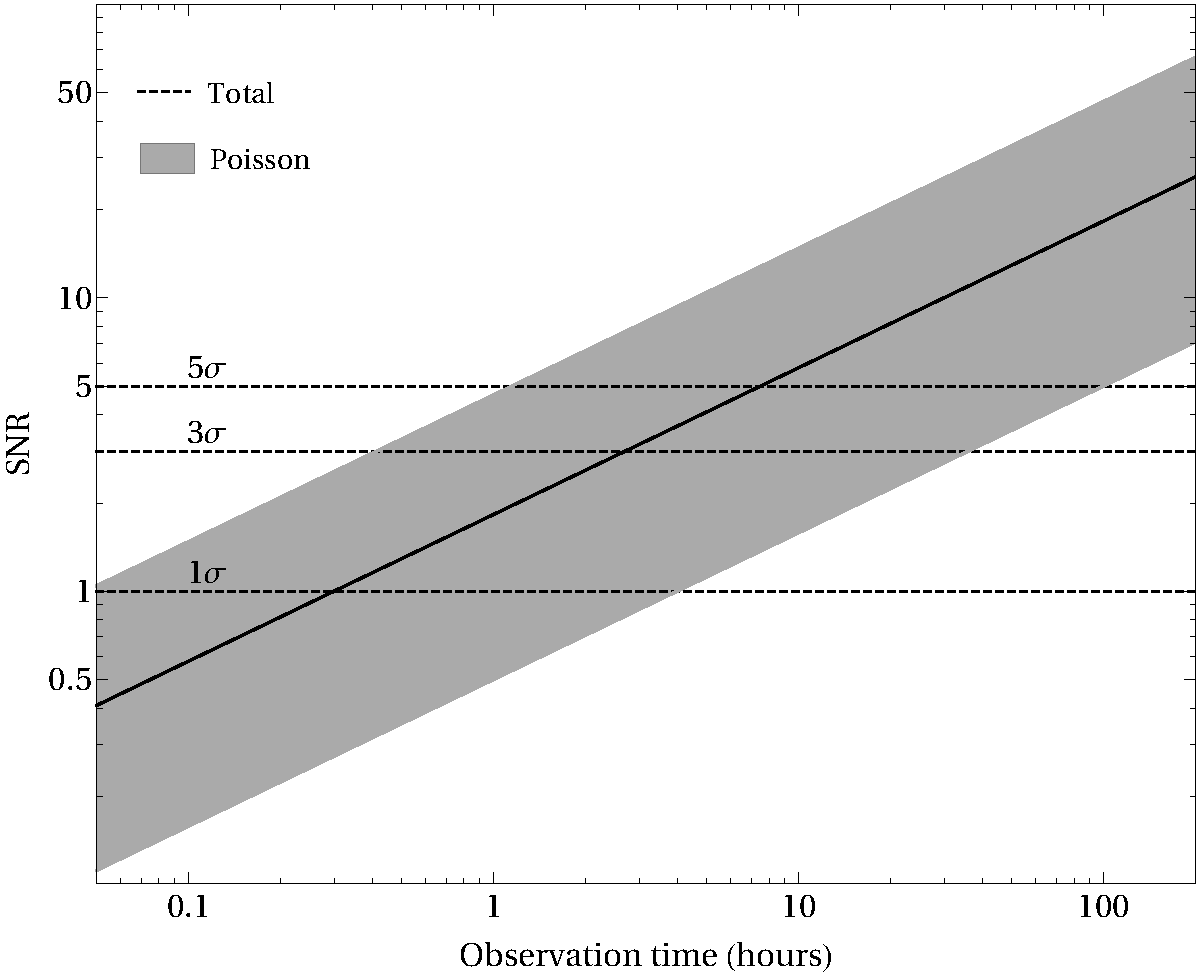
\includegraphics[width=\textwidth]{SNR-PBH-power.pdf}
    \bicaption[LISA探测器对探测原初双黑洞和双中子星产生的总的随机引力波背景的信噪比随观测时间的关系。原初黑洞的质量函数为幂率形式。黑色实线表示信噪比的中心值,而灰色区域表示信噪比的误差范围。对于双黑洞,我们固定$\al$和局域并合率$R$为其最佳拟合值,即$\al = 1.61$和$R = 80\,^{+108}_{-56}$\, $\gpcyr$。该情况下对应的原初黑洞占冷暗物质的丰度为$\fpbh = 3.8\,^{+2.3}_{-1.8} \times 10^{-3}$;而对于双中子星,我们取局域并合率为$R = 1540_{-1220}^{+3200}$\,$\gpcyr$。在大约观测$10$个小时后,LISA可以探测到中心值大小的总的随机引力波背景;探测的信噪比为$\mathrm{SNR}=5$。]{\label{SNR-PBH-power}
        LISA探测器对探测原初双黑洞和双中子星产生的总的随机引力波背景的信噪比随观测时间的关系。原初黑洞的质量函数为幂率形式。黑色实线表示信噪比的中心值,而灰色区域表示信噪比的误差范围。对于双黑洞,我们固定$\al$和局域并合率$R$为其最佳拟合值,即$\al = 1.61$和$R = 80\,^{+108}_{-56}$\, $\gpcyr$。该情况下对应的原初黑洞占冷暗物质的丰度为$\fpbh = 3.8\,^{+2.3}_{-1.8} \times 10^{-3}$;而对于双中子星,我们取局域并合率为$R = 1540_{-1220}^{+3200}$\,$\gpcyr$\citep{TheLIGOScientific:2017qsa}。在大约观测$10$个小时后,LISA可以探测到中心值大小的总的随机引力波背景;探测的信噪比为$\mathrm{SNR}=5$。
    }{The SNR of LISA as a function of observation time for median total 
        stochastic gravitational-wave background (black curve) and associated uncertainties (grey shaded region),
        from the primordial-origin binary black holes (with a \textit{power-law} mass function) and binary neutron stars.
        For binary black holes, we adopt the best-fit value for $\al = 1.61$, 
        and the inferred local merger rate $R = 80\,^{+108}_{-56}$\, $\gpcyr$,
        which corresponds to $\fpbh = 3.8\,^{+2.3}_{-1.8} \times 10^{-3}$. 
        And for binary neutron stars, we adopt $R = 1540_{-1220}^{+3200}$\,$\gpcyr$ 
        \citep{TheLIGOScientific:2017qsa}.
        The predicted median total background can be detected with 
        $\mathrm{SNR}=5$ after about $10$ hours of observation time.}
\end{figure}

\begin{figure}[htbp!]
    \centering
    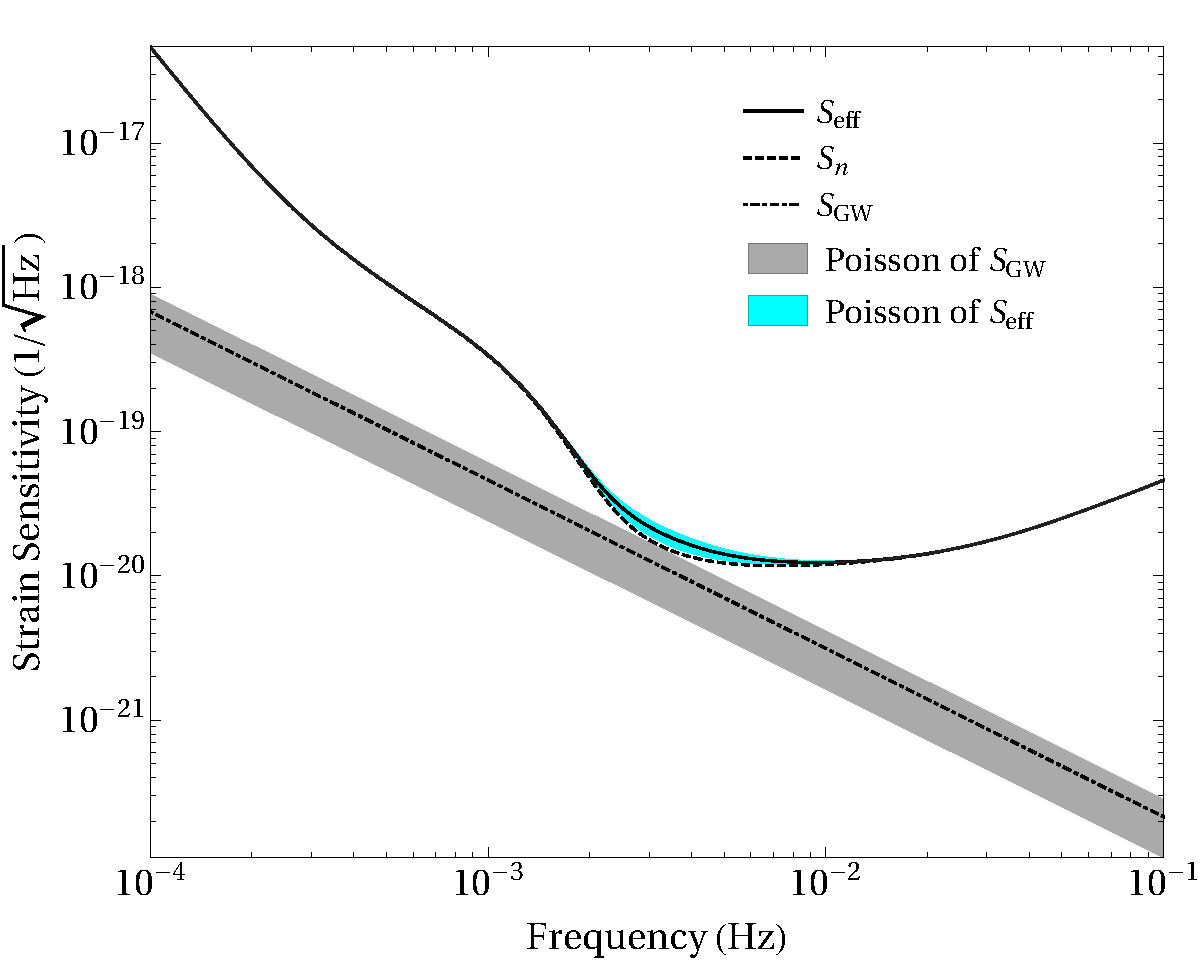
\includegraphics[width=\textwidth]{lisa-sensitivity-PBH-power.pdf}
    \bicaption{\label{lisa-sensitivity-PBH-power}
        由原初双黑洞和双中子星产生的总的随机引力波背景导致LISA探测器的有效应变灵敏度$S_{\mathrm{eff}}$(黑色实线)以及相应的泊松误差(青色区域)。原初黑洞的质量函数为幂率形式。图中还给出了LISA探测器的应变灵敏度$S_n$(虚线)以及引力波背景对应的应变灵敏度$S_{\mathrm{GW}}$(点虚线)和相应的泊松误差(灰色区域)。
    }{The effective strain sensitivity $S_{\mathrm{eff}}$ (black solid curve) of LISA
        and its Poisson uncertainties (cyan region),
        due to the effect of the total stochastic gravitational-wave background from primordial-origin binary black holes 
        (with a \textit{power-law} mass function) and binary neutron stars.
        We also show LISA's strain sensitivity $S_n$ (dashed curve),
        and $S_{\mathrm{GW}}$ (dot-dashed curve) 
        along with its Poisson uncertainties (grey shaded region).}
\end{figure}  

\begin{figure}[htbp!]
    \centering
    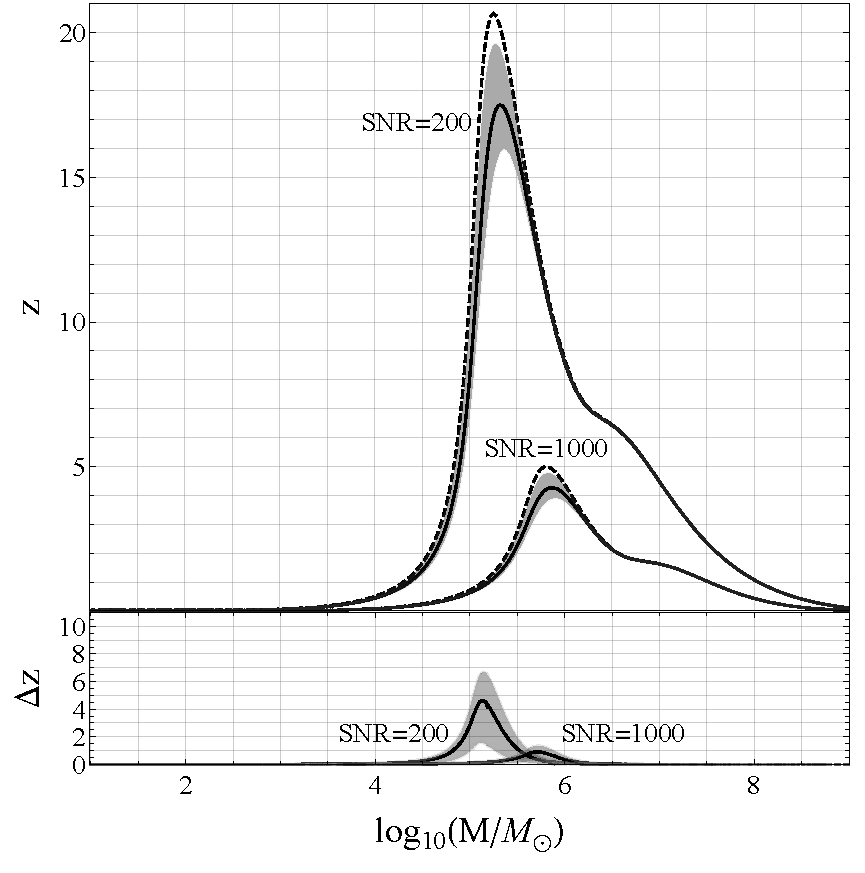
\includegraphics[width=\textwidth]{z-PBH-power.pdf}
    \bicaption[由原初双黑洞和双中子星产生的总的随机引力波背景对LISA探测器对于大质量双黑洞系统最大可探测红移$z$的影响。我们用$M$表示大质量双黑洞的总质量。原初黑洞的质量函数为幂率形式。我们固定质量比为$q=0.2$。我们分别考虑$\SNR=200$和$\SNR=1000$的两种情况。上图的虚线表示LISA最大可探测红移的等高线,而黑色实线表示考虑了随机引力波背景后LISA的最大可探测红移的等高线。灰色区域是黑色实线对应的泊松误差范围。下图给出了考虑随机引力波背景后对LISA最大可探测红移所引起的变化及误差范围。]{\label{z-PBH-power}
        由原初双黑洞和双中子星产生的总的随机引力波背景对LISA探测器对于大质量双黑洞系统最大可探测红移$z$的影响。我们用$M$表示大质量双黑洞的总质量。原初黑洞的质量函数为幂率形式。仿照\cite{Audley:2017drz},我们固定质量比为$q=0.2$。我们分别考虑$\SNR=200$和$\SNR=1000$的两种情况。上图的虚线表示LISA最大可探测红移的等高线,而黑色实线表示考虑了随机引力波背景后LISA的最大可探测红移的等高线。灰色区域是黑色实线对应的泊松误差范围。下图给出了考虑随机引力波背景后对LISA最大可探测红移所引起的变化及误差范围。
    }{The impacts of the total stochastic gravitational-wave background from primordial-origin binary black holes 
        (with a \textit{power-law} mass function) and binary neutron stars, 
        on the largest detectable redshift $z$ of MBHB (with total mass $M$) coalescences for LISA.
        The mass ratio is set to $q=0.2$ following \cite{Audley:2017drz}. 
        The upper panel shows the contours of $\SNR=200$ and $\SNR=1000$ 
        for LISA (dashed curves), 
        together with the effect of stochastic gravitational-wave background (black curves) and the Poisson error 
        bars (grey shaded region). 
        The lower panel shows the residuals of corresponding contours. }
\end{figure}

利用LIGO第一个观测阶段探测到的$3$个双黑洞并合事件,并考虑选择效应后,我们得到$\al$的最佳拟合值为$\al = 1.61$。固定$\al$的大小为其最佳拟合值,我们进而得到局域并合率$R$的中心值以及$90\%$的置信区间为$R = 80\,^{+108}_{-56}$\, $\gpcyr$。在\Fig{posterior-PBH-power}中,我们给出了$\al$和$R$的后验分布。从局域并合率$R$的后验分布,我们进一步得到原初黑洞占冷暗物质的丰度为$\fpbh = 3.8\,^{+2.3}_{-1.8} \times 10^{-3}$。我们的结果和之前的估算是一致的,即$10^{-3} \lesssim \fpbh \lesssim 10^{-2}$\citep{Sasaki:2016jop,Ali-Haimoud:2017rtz,Raidal:2017mfl,    Kocsis:2017yty,Chen:2018czv},从而验证了主要的冷暗物质不是由恒星级质量的原初黑洞构成的。



利用\Eq{OmegaGW},我们可以计算相应的随机引力波背景。\Fig{OmegaGW-PBH-power}给出了随机引力波背景的无量纲能量密度谱。从图上可以看出,随机引力波背景的强度可以超过LIGO设计阶段和LISA对应的灵敏度曲线,表明原初双黑洞和双中子星产生的随机引力波背景可以被LIGO设计阶段和LISA探测到。

在LIGO和LISA的可探测频段内,具有幂率质量分布的原初双黑洞和双中子星产生的引力波背景都近似和频率的$2/3$次方成正比,即$\ogw \propto \nu^{2/3}$。这是因为在可探测的频段内,随机引力波背景的贡献主要来自于双黑洞或双中子星的旋进阶段,而在旋进阶段,单个双黑洞或双中子星辐射的引力波能量谱大概就和频率的$2/3$次方成正比。在\Table{Omegaf-PBH-power}中,我们总结了在LIGO和LISA最灵敏的频率附近的随机引力波背景的能量密度的大小$\ogw (\nu)$。


\Fig{SNR-PBH-power}给出了预期累积信噪比关于时间的函数关系。由图可知,在观测$2$小时后,LISA可以探测到来自具有幂率质量分布的原初双黑洞和双中子星的中心值大小的随机引力波背景,相应的信噪比为$\mathrm{SNR} = 5$。在最乐观的情况下LISA观测$2$个小时就能探测到信噪比$\mathrm{SNR} = 5$的总的随机引力波背景,而在最悲观的情况下LISA观测$5$天能探测到信噪比$\mathrm{SNR} = 5$的总的随机引力波背景。


\Fig{lisa-sensitivity-PBH-power}给出了应变灵敏度曲线。\Fig{z-PBH-power}给出了随机引力波背景对LISA探测大质量双黑洞并合的信噪比的影响,表明最大可探测红移会由于未解析出来的随机引力波背景的影响而减小。这也表明LISA可探测的区域被压低了,从而减少LISA可探测到的大质量双黑洞并合的事件数。从\Fig{z-PBH-power}看出,由于随机引力波背景导致的等效噪音可以压低LISA对$10^5 \Msun$以上的种子黑洞并合的最大可探测红移。




\FloatBarrier
%%%%%%%%%%%%%%%%%%%%%%%%%%%%%%%%%%%%%%%%%%%%%%%%%%%%%%%%%%%%%%%%%%%%%%
\subsection{对数正态质量函数}

我们现在考虑对数正态的原初黑洞质量分布\citep{Dolgov:1992pu},
\e\label{log}
P(m) = \frac{1}{\sqrt{2 \pi} \s m} 
\exp\(-\frac{\ln^2(m/m_c)}{2 \s^2}\),
\q
其中$m_c$表征质量谱的峰值,而$\s$表征质量谱的宽度。在这种情况下,模型有三个自由参数,为$\{\vth, R\} = \{m_c, \s, R\}$.

\begin{figure}[htb!]
    \centering
    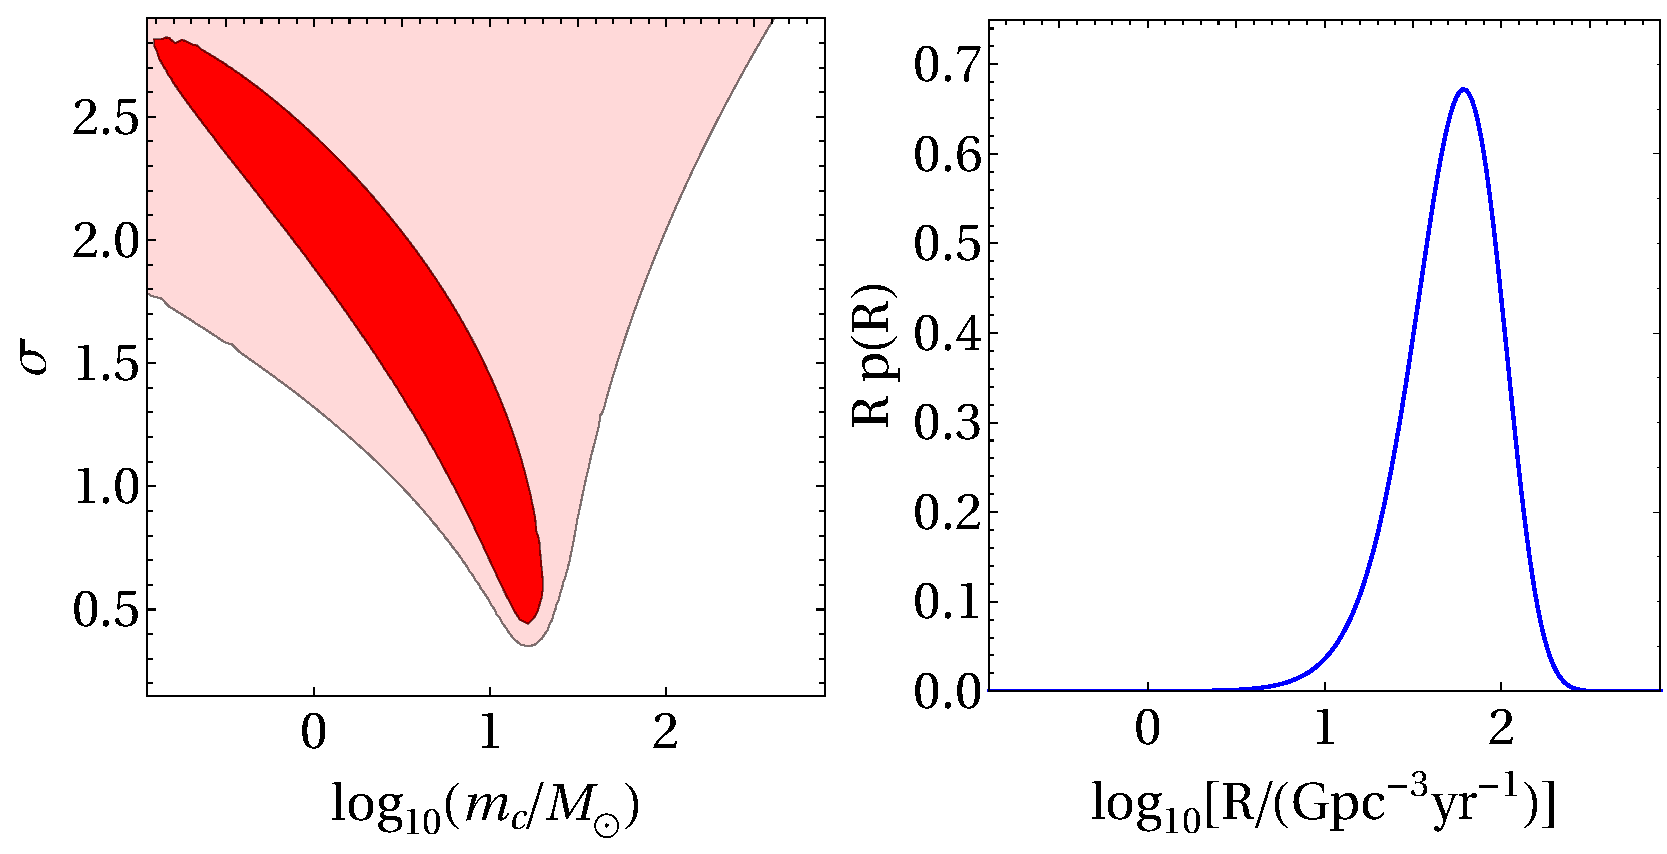
\includegraphics[width=\textwidth]{posterior-PBH-log.pdf}
    \bicaption{\label{posterior-PBH-log} 
        当原初黑洞质量函数为\textit{对数正态}形式的情况下,用LIGO第一个观测阶段的$3$个双黑洞并合事件拟合得到模型参数$\{\vth, R\} = \{m_c, \s, R\}$的一维和二维后验分布。左图的等高线分别对应$68\%$和$95\%$的置信区间。
    }{The posterior distributions for $\{\vth, R\} = \{m_c, \s, R\}$ of
    \textit{lognormal} mass function for primordial black holes, at the $68\%$ and $95\%$ 
    credible level, respectively, by using $3$ events from 
    LIGO's O1 observing run.  }
\end{figure}

利用LIGO第一个观测阶段探测到的$3$个双黑洞并合事件,并考虑选择效应后,我们得到$m_c$和$\s$的最佳拟合值为$\{m_c, \s\} = \{14.8 \Msun, 0.65\}$。固定$m_c$和$\s$的大小为其最佳拟合值,我们进而得到局域并合率$R$的中心值以及$90\%$的置信区间为$R = 55\,^{+74}_{-38}$\, $\gpcyr$。在\Fig{posterior-PBH-log}中,我们给出了$m_c$、$\s$和$R$的后验分布。从局域并合率$R$的后验分布,我们进一步得到原初黑洞占冷暗物质的丰度为$\fpbh = 2.8\,^{+1.6}_{-1.3} \times 10^{-3}$。我们的结果和之前的估算是一致的,即$10^{-3} \lesssim \fpbh \lesssim 10^{-2}$\citep{Sasaki:2016jop,Ali-Haimoud:2017rtz,Raidal:2017mfl,    Kocsis:2017yty,Chen:2018czv},从而验证了主要的冷暗物质不是由恒星级质量的原初黑洞构成的。

\begin{figure}[htbp!]
    \centering
    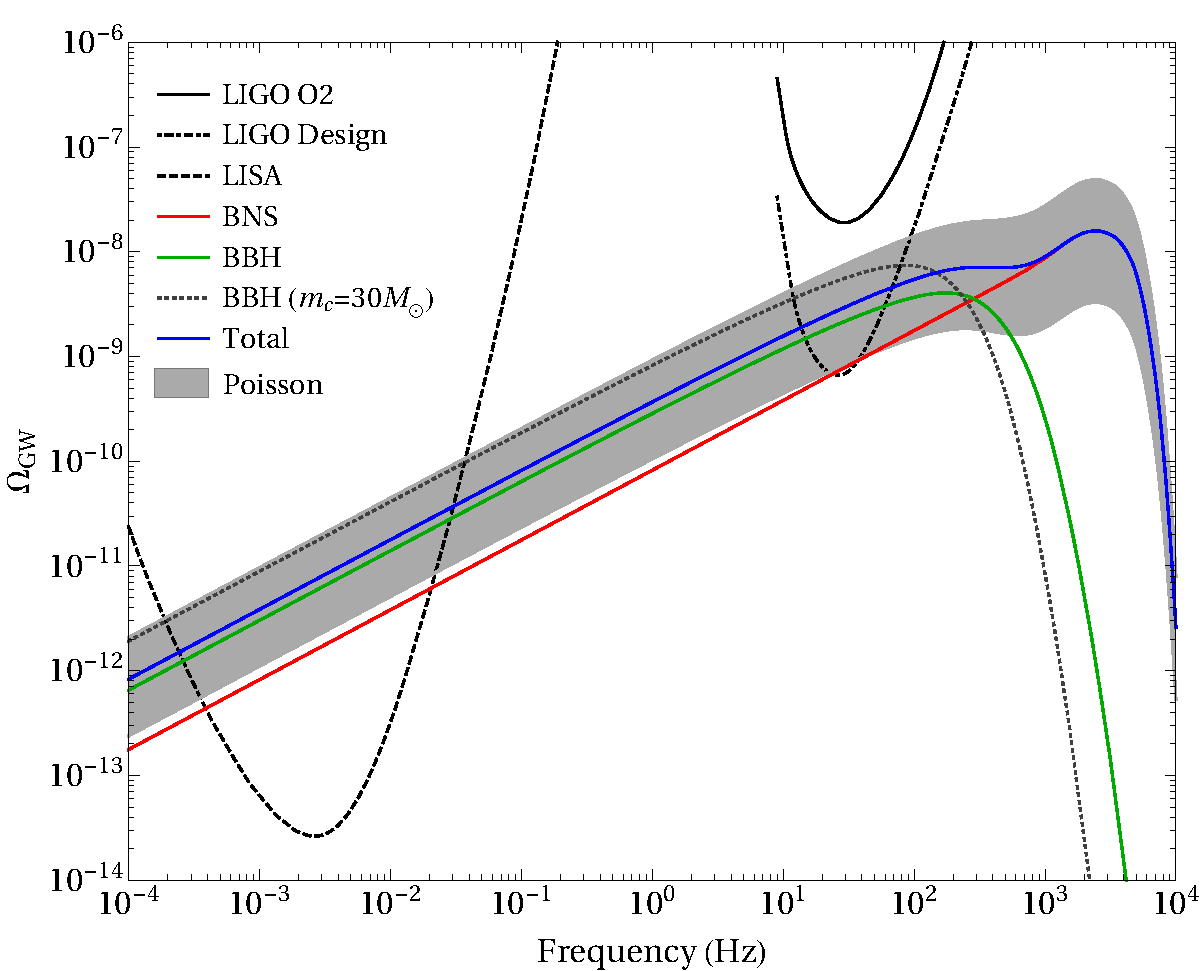
\includegraphics[width=0.8\textwidth]{OmegaGW-PBH-log.pdf}
    \bicaption[来自对数正态质量分布的原初双黑洞和双中子星产生的随机引力波背景。绿线是双黑洞对应的随机引力波背景,而红线是双中子星对应的随机引力波背景。蓝色表示总的引力波背景;灰色区域则表示总的随机引力波背景的泊松误差。对于双黑洞,我们固定$\{m_c, \s\}$和局域并合率$R$为其最佳拟合值,即$\{m_c, \s\} = \{14.8\, \Msun,\,0.65\}$和$R = 55\,^{+74}_{-38}$\, $\gpcyr$。该情况下对应的原初黑洞占冷暗物质的丰度为$\fpbh = 2.8\,^{+1.6}_{-1.3} \times 10^{-3}$;而对于双中子星,我们取局域并合率为$R = 1540_{-1220}^{+3200}$\,$\gpcyr$。图中的黑色实线表示LIGO第二个观测阶段(O2)的幂率积分曲线;点虚线表示LIGO设计阶段对应的幂率积分曲线;而虚线则表示LISA观测四年对应的幂率积分曲线。LIGO设计阶段和LISA对应的幂率积分曲线都能跨过泊松误差区域,表明原初双黑洞和双中子星产生的随机引力波背景可以被LIGO设计阶段和LISA探测到。]{\label{OmegaGW-PBH-log} 
        来自对数正态质量分布的原初双黑洞和双中子星产生的随机引力波背景。绿线是双黑洞对应的随机引力波背景,而红线是双中子星对应的随机引力波背景。蓝色表示总的引力波背景;灰色区域则表示总的随机引力波背景的泊松误差。对于双黑洞,我们固定$\{m_c, \s\}$和局域并合率$R$为其最佳拟合值,即$\{m_c, \s\} = \{14.8\, \Msun,\,0.65\}$和$R = 55\,^{+74}_{-38}$\, $\gpcyr$,且$\fpbh = 2.8\,^{+1.6}_{-1.3} \times 10^{-3}$;而对于双中子星,我们取局域并合率为$R = 1540_{-1220}^{+3200}$\,$\gpcyr$\citep{TheLIGOScientific:2017qsa}。图中的黑色实线表示LIGO第二个观测阶段(O2)的幂率积分曲线;点虚线表示LIGO设计阶段对应的幂率积分曲线;而虚线则表示LISA观测四年对应的幂率积分曲线。LIGO设计阶段和LISA对应的幂率积分曲线都能跨过泊松误差区域,表明原初双黑洞和双中子星产生的随机引力波背景可以被LIGO设计阶段和LISA探测到。
    }{The predicted stochastic gravitational-wave background from the binary neutron stars and primordial-origin binary black holes
    with a \textit{lognormal} mass function. 
    The red and green curves are backgrounds from the binary neutron stars (BNSs) and binary black holes (BBHs), respectively. 
    The total background is shown in the blue curve, while
    its Poisson error bars are in the grey shaded region.
    For binary black holes, we adopt the best-fit values for 
    $\{m_c, \s\} = \{14.8\, \Msun,\,0.65\}$, 
    and the inferred local merger rate $R = 55\,^{+74}_{-38}$\, $\gpcyr$,
    which corresponds to $\fpbh = 2.8\,^{+1.6}_{-1.3} \times 10^{-3}$.
    And for binary neutron stars, we adopt $R = 1540_{-1220}^{+3200}$\,$\gpcyr$ 
    \citep{TheLIGOScientific:2017qsa}.
    The dotted line shows the background from binary black holes with $m_c = 30 \Msun$, 
    by fixing $\s = 0.65$ and $R = 55$\, $\gpcyr$.
    We also show the expected PI curves for LISA with $4$ years of 
    observation (dashed) and
    LIGO's O2 (black) and design sensitivity (dot-dashed).
    The PI curves for LISA and LIGO's design sensitivity cross the Poisson
    error region, indicating the possibility to detect this background.}
\end{figure}

\begin{table}[htb!]
    \centering
    \begin{tabular}{c|c|c}
        &\ $\Omega_{\mathrm{GW}}(25 \, \mathrm{Hz})$ \
        &\ $\Omega_{\mathrm{GW}}(3 \times 10^{-3} \, \mathrm{Hz})$\,\\
        \hline
        BNS\, &  $0.7^{+1.5}_{-0.6} \times 10^{-9}$ 
        & $1.7^{+3.5}_{-1.4} \times 10^{-12}$ \\
        [.3em]
        \hline
        BBH\, & $2.0^{+2.7}_{-1.4} \times 10^{-9}$  
        & $6.3^{+8.5}_{-4.2} \times 10^{-12}$ \\
        [.3em]
        \hline
        Total\, & $2.7^{+4.2}_{-2.0} \times 10^{-9}$  
        & $8.0^{+12}_{-5.6} \times 10^{-12}$ \\
        [.2em]
    \end{tabular}
    \bicaption{\label{Omegaf-PBH-log}
        原初双黑洞产生的随机引力波背景、双中子星产生的随机引力波背景以及总的随机引力波背景在LIGO和LISA最灵敏的频率附近(分别为$25 \, \mathrm{Hz}$和$3 \times 10^{-3} \, \mathrm{Hz}$)的大小。原初黑洞质量函数为对数正态形式。我们还给出了$90\%$的泊松误差范围。
    }{Estimates of the background energy density $\ogw (\nu)$ at the most sensitive frequencies of LIGO (near $25$ Hz) and LISA (near $3\times 10^{-3}$ Hz) for each of the binary neutron star (BNS), primordial-origin binary black hole (BBH, with a \textit{lognormal} mass function) and total background contributions, along with the $90\%$ Poisson error bounds.}
\end{table}

\begin{figure}[htbp!]
    \centering
    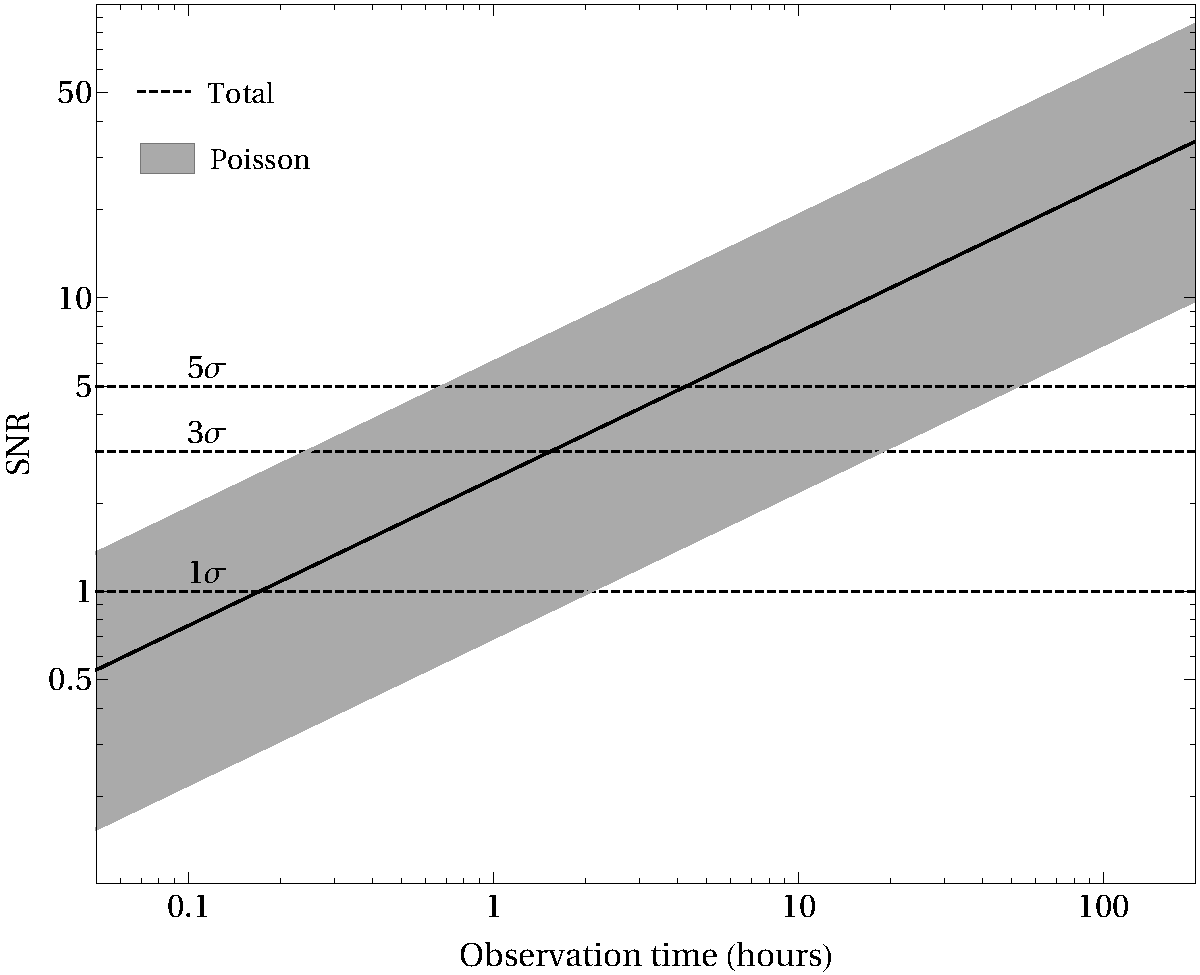
\includegraphics[width=\textwidth]{SNR-PBH-log.pdf}
    \bicaption[LISA探测器对探测原初双黑洞和双中子星产生的总的随机引力波背景的信噪比随观测时间的关系。原初黑洞质量函数为对数正态形式。黑色实线表示信噪比的中心值,而灰色区域表示信噪比的误差范围。对于双黑洞,我们固定$\{m_c, \s\}$和局域并合率$R$为其最佳拟合值,即$\{m_c, \s\} = \{14.8\, \Msun,\,0.65\}$和$R = 55\,^{+74}_{-38}$\, $\gpcyr$。该情况下对应的原初黑洞占冷暗物质的丰度为$\fpbh = 2.8\,^{+1.6}_{-1.3} \times 10^{-3}$;而对于双中子星,我们取局域并合率为$R = 1540_{-1220}^{+3200}$\,$\gpcyr$。在大约观测$5$个小时后,LISA可以探测到中心值大小的总的随机引力波背景;探测的信噪比为$\mathrm{SNR}=5$。]{\label{SNR-PBH-log} 
        LISA探测器对探测原初双黑洞和双中子星产生的总的随机引力波背景的信噪比随观测时间的关系。原初黑洞质量函数为对数正态形式。黑色实线表示信噪比的中心值,而灰色区域表示信噪比的误差范围。对于双黑洞,我们固定$\{m_c, \s\}$和局域并合率$R$为其最佳拟合值,即$\{m_c, \s\} = \{14.8\, \Msun,\,0.65\}$和$R = 55\,^{+74}_{-38}$\, $\gpcyr$。该情况下对应的原初黑洞占冷暗物质的丰度为$\fpbh = 2.8\,^{+1.6}_{-1.3} \times 10^{-3}$;而对于双中子星,我们取局域并合率为$R = 1540_{-1220}^{+3200}$\,$\gpcyr$\citep{TheLIGOScientific:2017qsa}。在大约观测$5$个小时后,LISA可以探测到中心值大小的总的随机引力波背景;探测的信噪比为$\mathrm{SNR}=5$。
    }{The SNR of LISA as a function of observation time for median total 
    stochastic gravitational-wave background (black curve) and associated uncertainties (grey shaded region),
    from primordial-origin binary black holes (with a \textit{lognormal} mass function) and binary neutron stars.
    Here, we adopt the best-fit values for 
    $\{m_c, \s\} = \{14.8\, \Msun,\,0.65\}$, 
    and the inferred local merger rate $R = 55\,^{+74}_{-38}$\, $\gpcyr$,
    which corresponds to $\fpbh = 2.8\,^{+1.6}_{-1.3} \times 10^{-3}$.
    The predicted median total background can be detected with 
    $\mathrm{SNR}=5$ after about $5$ hours of observation time.}
\end{figure}

利用\Eq{OmegaGW},我们可以计算相应的随机引力波背景。\Fig{OmegaGW-PBH-log}给出了随机引力波背景的无量纲能量密度谱。从图上可以看出,随机引力波背景的强度可以超过LIGO设计阶段和LISA对应的灵敏度曲线,表明原初双黑洞和双中子星产生的随机引力波背景可以被LIGO设计阶段和LISA探测到。

在LIGO和LISA的可探测频段内,具有对数正态质量分布的原初双黑洞和双中子星产生的引力波背景都近似和频率的$2/3$次方成正比,即$\ogw \propto \nu^{2/3}$。这是因为在可探测的频段内,随机引力波背景的贡献主要来自于双黑洞或双中子星的旋进阶段,而在旋进阶段,单个双黑洞或双中子星辐射的引力波能量谱大概就和频率的$2/3$次方成正比。在\Table{Omegaf-PBH-log}中,我们总结了在LIGO和LISA最灵敏的频率附近的随机引力波背景的能量密度的大小$\ogw (\nu)$。



\begin{figure}[htbp!]
    \centering
    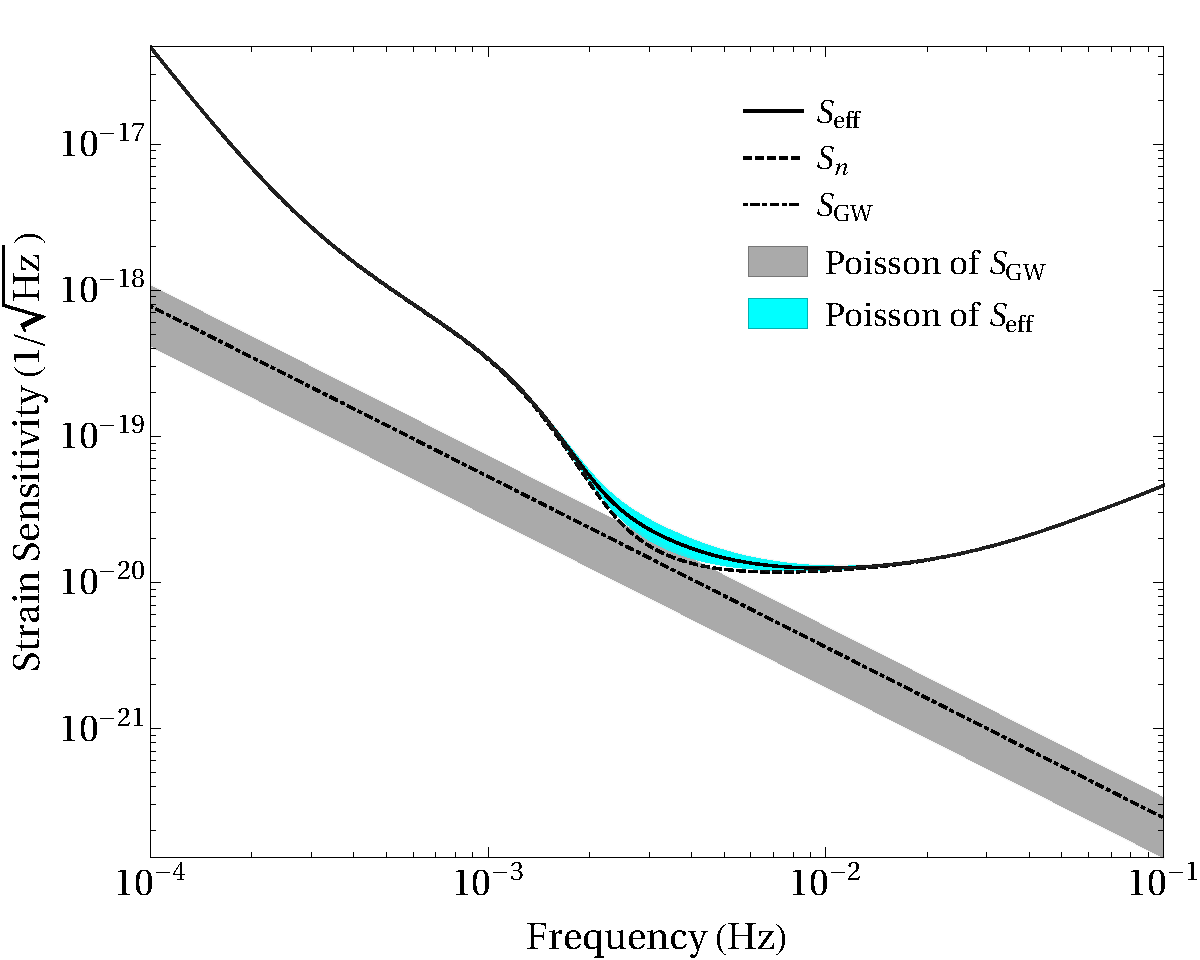
\includegraphics[width=\textwidth]{lisa-sensitivity-PBH-log.pdf}
    \bicaption{\label{lisa-sensitivity-PBH-log}        
        由原初双黑洞和双中子星产生的总的随机引力波背景导致LISA探测器的有效应变灵敏度$S_{\mathrm{eff}}$(黑色实线)以及相应的泊松误差(青色区域)。原初黑洞质量函数为对数正态形式。图中还给出了LISA探测器的应变灵敏度$S_n$(虚线)以及引力波背景对应的应变灵敏度$S_{\mathrm{GW}}$(点虚线)和相应的泊松误差(灰色区域)。
    }{The effective strain sensitivity $S_{\mathrm{eff}}$ (black solid curve) of LISA
    and its Poisson uncertainties (cyan region),
    due to the effect of the total stochastic gravitational-wave background from primordial-origin binary black holes 
    (with a \textit{log-normal} mass function) and binary neutron stars.
    We also show LISA's strain sensitivity $S_n$ (dashed curve),
    and $S_{\mathrm{GW}}$ (dot-dashed curve) 
    along with its Poisson uncertainties (grey shaded region).}
\end{figure}  



\begin{figure}[htbp!]
    \centering
    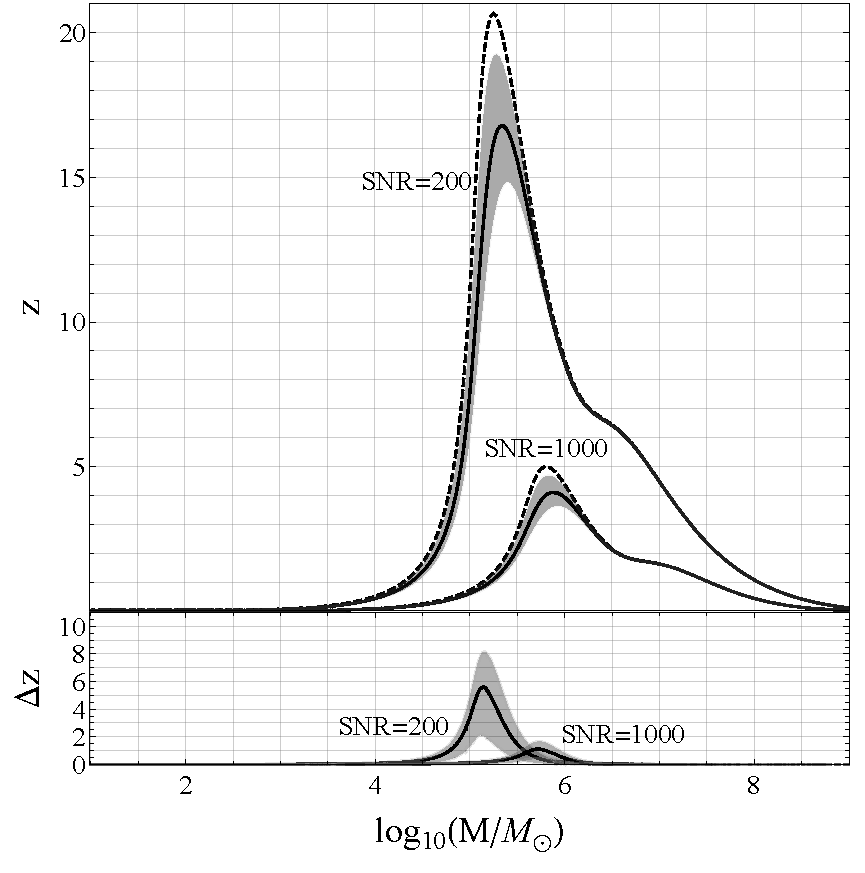
\includegraphics[width=\textwidth]{z-PBH-log.pdf}
    \bicaption[由原初双黑洞和双中子星产生的总的随机引力波背景对LISA探测器对于大质量双黑洞系统最大可探测红移$z$的影响。我们用$M$表示大质量双黑洞的总质量。原初黑洞质量函数为对数正态形式。仿照,我们固定质量比为$q=0.2$。我们分别考虑$\SNR=200$和$\SNR=1000$的两种情况。上图的虚线表示LISA最大可探测红移的等高线,而黑色实线表示考虑了随机引力波背景后LISA的最大可探测红移的等高线。灰色区域是黑色实线对应的泊松误差范围。下图给出了考虑随机引力波背景后对LISA最大可探测红移所引起的变化及误差范围。]{\label{z-PBH-log}
        由原初双黑洞和双中子星产生的总的随机引力波背景对LISA探测器对于大质量双黑洞系统最大可探测红移$z$的影响。我们用$M$表示大质量双黑洞的总质量。原初黑洞质量函数为对数正态形式。仿照\cite{Audley:2017drz},我们固定质量比为$q=0.2$。我们分别考虑$\SNR=200$和$\SNR=1000$的两种情况。上图的虚线表示LISA最大可探测红移的等高线,而黑色实线表示考虑了随机引力波背景后LISA的最大可探测红移的等高线。灰色区域是黑色实线对应的泊松误差范围。下图给出了考虑随机引力波背景后对LISA最大可探测红移所引起的变化及误差范围。
    }{The impacts of the total stochastic gravitational-wave background from primordial-origin binary black holes 
    (with a \textit{lognormal} mass function) and binary neutron stars, 
    on the largest detectable redshift $z$ of MBHB (with total mass $M$) coalescences for LISA.
    The mass ratio is set to $q=0.2$ following \cite{Audley:2017drz}. 
    The upper panel shows the contours of $\SNR=200$ and $\SNR=1000$ 
    for LISA (dashed curves), 
    together with the effect of stochastic gravitational-wave background (black curves) and the Poisson error 
    bars (grey shaded region). 
    The lower panel shows the residuals of corresponding contours. }
\end{figure}


\Fig{SNR-PBH-log}给出了预期累积信噪比关于时间的函数关系。由图可知,在观测$5$小时后,LISA可以探测到来自具有对数正态质量分布的原初双黑洞和双中子星的中心值大小的随机引力波背景,相应的信噪比为$\mathrm{SNR} = 5$。在最乐观的情况下LISA观测$1$个小时就能探测到信噪比$\mathrm{SNR} = 5$的总的随机引力波背景,而在最悲观的情况下LISA观测$3$天能探测到信噪比$\mathrm{SNR} = 5$的总的随机引力波背景。

\Fig{lisa-sensitivity-PBH-log}给出了应变灵敏度曲线。\Fig{z-PBH-log}给出了随机引力波背景对LISA探测大质量双黑洞并合的信噪比的影响,表明最大可探测红移会由于未解析出来的随机引力波背景的影响而减小。这也表明LISA可探测的区域被压低了,从而减少LISA可探测到的大质量双黑洞并合的事件数。从\Fig{z-PBH-log}看出,由于随机引力波背景导致的等效噪音可以压低LISA对$10^5 \Msun$以上的种子黑洞并合的最大可探测红移。



%%%%%%%%%%%%%%%%%%%%%%%%%%%%%%%%%%%%%%%%%%%%%%%%%%%%%%%%%%%%%%%%%%%%%%
\section{总结和讨论}

在本章中,我们计算了来自双黑洞和双中子星并合产生的随机引力波背景。而且探究了这一随机引力波背景对LISA空间引力波探测器探测能力的影响。我们考虑了两种不同的双黑洞形成机制,分别是天体物理双黑洞和原初双黑洞机制。

对于天体物理黑洞,我们采用了被广泛接受的``\textit{Vangioni}"模型\citep{Dvorkin:2016wac}。而对于原初黑洞,我们考虑了两种流行的迥异的原初黑洞质量谱,分别为幂率质量分布和对数正态质量分布。对于幂率质量谱的情况,我们从LIGO的引力波数据分析得到局域并合率为$R = 80\,^{+108}_{-56}$\, $\gpcyr$,相应的原初黑洞占冷暗物质的丰度为$\fpbh = 3.8\,^{+2.3}_{-1.8} \times 10^{-3}$。对于对数正态的质量谱,我们得到$R = 55\,^{+74}_{-38}$\, $\gpcyr$,对应于$\fpbh = 2.8\,^{+1.6}_{-1.3} \times 10^{-3}$。由于幂率形式的质量谱会给出更多的轻质量的原初黑洞,所以相较对数正态质量分布而言,为了和\lvc 相自洽,其预言的局域并合率要大一些。之前文献\citep{Kawasaki:2016jop,Ali-Haimoud:2017rtz,Raidal:2017mfl,Kocsis:2017yty,Chen:2018czv}中对原初黑洞占冷暗物质的估计大约为$10^{-3} \lesssim \fpbh \lesssim 10^{-2}$。对于这两种原初黑洞的质量谱,我们推断得到的原初黑洞的丰度和之前的估计一致的,从而验证了主要的冷暗物质不是由恒星级质量的原初黑洞构成的。

我们发现原初双黑洞产生的随机引力波背景要比天体物理双黑洞产生的随机引力波背景要强(见\Fig{OmegaGW-sBH}、\Fig{OmegaGW-PBH-power}、\Fig{OmegaGW-PBH-log}以及\Table{Omegaf-sBH}、\Table{Omegaf-PBH-power}、\Table{Omegaf-PBH-log})。这是由于原初双黑洞和天体物理双黑洞的并合率随黑洞的质量和红移的关系不同导致的。特别是,原初双黑洞的并合率会随着红移的增长而快速增长;而天体物理双黑洞的并合率则随着红移先增长,接着在红移为$z \sim 1-2$附近达到峰值,然后急剧速减小。我们还发现,在\lvc 和LISA灵敏的频段内,不管是天体物理双黑洞还是原初双黑洞形成的随机引力波背景的能量密度谱都和频率成$2/3$次方的关系,即$\ogw \propto \nu^{2/3}$。所以用\lvc 和LISA通过探测随机引力波背景的方法将很难区分到底是是天体物理双黑洞还是原初双黑洞形成的随机引力波背景。

最后,我们发现由双黑洞和双中子星形成的总的随机引力波背景很可能被未来的引力波探测器\lvc 和LISA探测到(见\Fig{OmegaGW-sBH}、\Fig{SNR-sBH}、\Fig{OmegaGW-PBH-power}、\Fig{SNR-PBH-power}、\Fig{OmegaGW-PBH-log}、\Fig{SNR-PBH-log})。这些随机引力波背景如果不从噪音背景中扣除掉的话,会成为LISA的额外噪音源(见\Fig{lisa-sensitivity-sBH}、\Fig{lisa-sensitivity-PBH-power}、\Fig{lisa-sensitivity-PBH-log}),从而弱化LISA的探测能力。例如,探测大质量双黑洞的并合是LISA的一个关键科学目标。由于随机引力波背景的影响,会压低LISA对于大质量双黑洞的最大可探测红移(见\Fig{z-sBH}、\Fig{z-PBH-power}、\Fig{z-PBH-log})。所以,为了提高探测器的探测能力,需要将随机引力波背景从LISA的噪音中扣除掉。